\newpage
\section{Appendix}
\label{sec:appendix}

{\small\setlength{\tabcolsep}{0pt}%
\begin{tabular}{@{}p{0.90\linewidth}r@{}}
  \hyperref[app:related_work]{\S\ref*{app:related_work}\enspace Comparison with Related Work}                                               & \pageref{app:related_work}    \\[2pt]
  \hyperref[app:limitations]{\S\ref*{app:limitations}\enspace Limitations and Future Work}                                                   & \pageref{app:limitations}     \\[2pt]
  \hyperref[app:qualitative_rollouts]{\S\ref*{app:qualitative_rollouts}\enspace Additional Qualitative Rollouts}                                                                    & \pageref{app:qualitative_rollouts}           \\[2pt]
  \hyperref[app:vocab]{\S\ref*{app:vocab}\enspace Full Action Vocabulary}                                                                    & \pageref{app:vocab}           \\[2pt]
  \hyperref[app:baseline_prompt]{\S\ref*{app:baseline_prompt}\enspace Baseline Prompt Settings}                                              & \pageref{app:baseline_prompt} \\[2pt]
  \hyperref[app:setup_details]{\S\ref*{app:setup_details}\enspace Experimental Setup Details}                                                & \pageref{app:setup_details}   \\[2pt]
  \hyperref[app:reliability]{\S\ref*{app:reliability}\enspace Annotator Reliability}                                                         & \pageref{app:reliability}     \\[2pt]
  \hyperref[app:stage1_ablation]{\S\ref*{app:stage1_ablation}\enspace Stage~$\mathbf{1}$: Conditioning Architecture Ablation}                & \pageref{app:stage1_ablation} \\[2pt]
  \hyperref[app:stage2_ablation]{\S\ref*{app:stage2_ablation}\enspace Stage~$\mathbf{2}$: KV-Cache and Bounded RoPE Ablation}                & \pageref{app:stage2_ablation} \\[2pt]
  \hyperref[app:stronger_id]{\S\ref*{app:stronger_id}\enspace Stronger Action-Index Baselines Collapse into NL}                              & \pageref{app:stronger_id}     \\[2pt]
  \hyperref[app:full_indist]{\S\ref*{app:full_indist}\enspace Axis~$\mathbf{1}$: Full In-Distribution Score Distributions}                   & \pageref{app:full_indist}     \\[2pt]
  \hyperref[app:axis2_tiers]{\S\ref*{app:axis2_tiers}\enspace Axis~$\mathbf{2}$: Full Cross-Entity Distributions and Per-Tier Mechanism}     & \pageref{app:axis2_tiers}     \\[2pt]
  \hyperref[app:oov_probes]{\S\ref*{app:oov_probes}\enspace OOV Probe Set}                                                                  & \pageref{app:oov_probes}      \\[2pt]
  \hyperref[app:failure]{\S\ref*{app:failure}\enspace Failure Case Analysis}                                                                 & \pageref{app:failure}         \\[2pt]
  \hyperref[app:long_horizon]{\S\ref*{app:long_horizon}\enspace Long-Horizon Stability}                                                      & \pageref{app:long_horizon}    \\[2pt]
    \hyperref[app:persistent_state]{\S\ref*{app:persistent_state}\enspace Extension: Persistent Entity State via an Observer--Tracker--Policy Loop} & \pageref{app:persistent_state}\\[2pt]
  \hyperref[app:realtime_pipeline]{\S\ref*{app:realtime_pipeline}\enspace Realtime Pipeline} & \pageref{app:realtime_pipeline}\\
\end{tabular}}\par\vspace{4pt}

\subsection{Comparison with Related Work}
\label{app:related_work}

\begin{table}[t]
  \caption{Systematic comparison of interactive video world models. 
  \cmark~=~supported, \xmark~=~not supported, $\sim$~=~partial. 
  \emph{Multi-entity} requires independent and simultaneous control of two 
  distinct entities. 
  \emph{Semantic NL} requires per-frame natural language action 
  conditioning.}
  \label{tab:comparison}
  \centering
  \begin{tabular}{lcccc}
    \toprule
    Model & Multi-entity & Semantic NL & $\geq$$16$FPS & $>$$5$min \\
    \midrule
    GameNGen~\citep{valevski2024diffusion}     & \xmark & \xmark & \cmark & \cmark \\
    Genie~$2$~\citep{parkerholder2024genie2}     & $\sim$ & \xmark & \cmark & \xmark \\
    Genie~$3$~\citep{parkerholder2025genie3}     & $\sim$ & \xmark & \cmark & $\sim$ \\
    The Matrix~\citep{feng2024matrix}          & \xmark & \xmark & \cmark & \cmark \\
    Matrix-Game $2.0$~\citep{he2025matrixgame2}  & \xmark & \xmark & \cmark & $\sim$ \\
    LingBot-World~\citep{team2026advancing}  & \xmark & \xmark & \cmark & \cmark \\
    Solaris~\citep{solaris2025}                & \cmark & \xmark & $\sim$ & $\sim$ \\
    \midrule
    \textbf{\methodname (Ours)}                & \cmark & \cmark & \cmark & \cmark \\
    \bottomrule
  \end{tabular}
\end{table}

Table~\ref{tab:comparison} presents a systematic comparison of 
\methodname against representative interactive video world models 
along four dimensions: multi-entity control, 
semantic natural language interface, 
real-time frame rate ($\geq$$16$FPS), and long-horizon 
generation ($>$$5$min).

\paragraph{Explanation of absence of world model baselines.}
As established in Table~\ref{tab:comparison} and 
Section~\ref{sec:related}, 
while a small number of existing world models 
accommodate concurrent multi-entity modeling to 
some extent, 
none achieves independent and simultaneous control 
of multiple entities within a single holistic scene. 
Because \methodname is, to our knowledge, 
the first system to address this setting, 
no directly comparable baseline exists for 
quantitative evaluation.

\paragraph{Additional Related Work for Efficient Streaming Video Generation. }
Several lines of work advance streaming video generation from complementary angles.
On the diffusion side, Flow Matching~\citep{lipman2022flow} and Distribution Matching Distillation (DMD)~\citep{yin2024one} substantially reduce the number of inference steps.
On the autoregressive side, Self-Forcing~\citep{chen2025selfforcing} eliminates exposure bias caused by the training-inference discrepancy.
For long-horizon memory management, StreamingLLM~\citep{xiao2023streamingllm} and LM-Infinite~\citep{han2023lminfinite} bound memory usage via attention-sink tokens and sliding-window KV caches.
Our work integrates these advances together to achieve real-time long-horizon streaming generation.

\subsection{Limitations and Future Work}
\label{app:limitations}

\methodname has three limitations that point toward concrete future directions.
First, our training labels are obtained by direct in-engine memory instrumentation, since games are the only domain that simultaneously offers frame-accurate, per-entity, zero-cost supervision at interactive frame rates; this is a deliberate testbed choice and is orthogonal to the language interface itself, which only consumes per-entity action captions and is agnostic to how those captions are produced. Closing the annotation channel for non-instrumented domains, namely real-world video and closed-source engines, reduces to producing per-entity captions from an alternative source such as vision--language auto-labelers, tele-operation logs, or robot proprioception, all of which integrate without architectural change. We therefore view this as a data-side problem rather than a structural restriction of \methodname.
Second, open-vocabulary expressiveness is ultimately bounded by the pretrained text encoder: composing concepts already within its training distribution generalizes naturally to unseen combinations, whereas truly novel tokens require explicit encoder adaptation. Our current interface also targets semantic action control rather than numerically precise continuous controls, such as camera $\mathrm{SE}(3)$ trajectories or force/velocity commands in robotic manipulation. This does not require replacing the language interface: a natural extension is to keep language as the high-level per-entity semantic channel and add a parallel continuous-control module, whose embeddings can be fused with the same per-frame conditioning layers used by \methodname.
Third, episode-level state beyond the generator's ${\sim}1.75$\,s context window is maintained by a hand-specified persistent-state module (Appendix~\ref{app:persistent_state}); replacing it with a learned, world-agnostic alternative remains open.
In strictly single-agent scenarios, the language interface also degenerates into a relabelling of discrete inputs and offers no representational advantage over conventional action identifiers.
Extending \methodname to non-game interactive-video domains, where per-entity annotations must be inferred rather than read from engine memory, constitutes the most immediate direction for future work.


\subsection{Additional Qualitative Rollouts}
\label{app:qualitative_rollouts}
We include additional qualitative rollouts to make the generated interactive worlds easier to inspect visually.
Figures~\ref{fig:margit_rollout_1min} and~\ref{fig:kof_rollout_0} complement the quantitative evaluation by showing representative long-horizon behavior in the two domains used in the paper.

\begin{figure}[h]
    \centering
    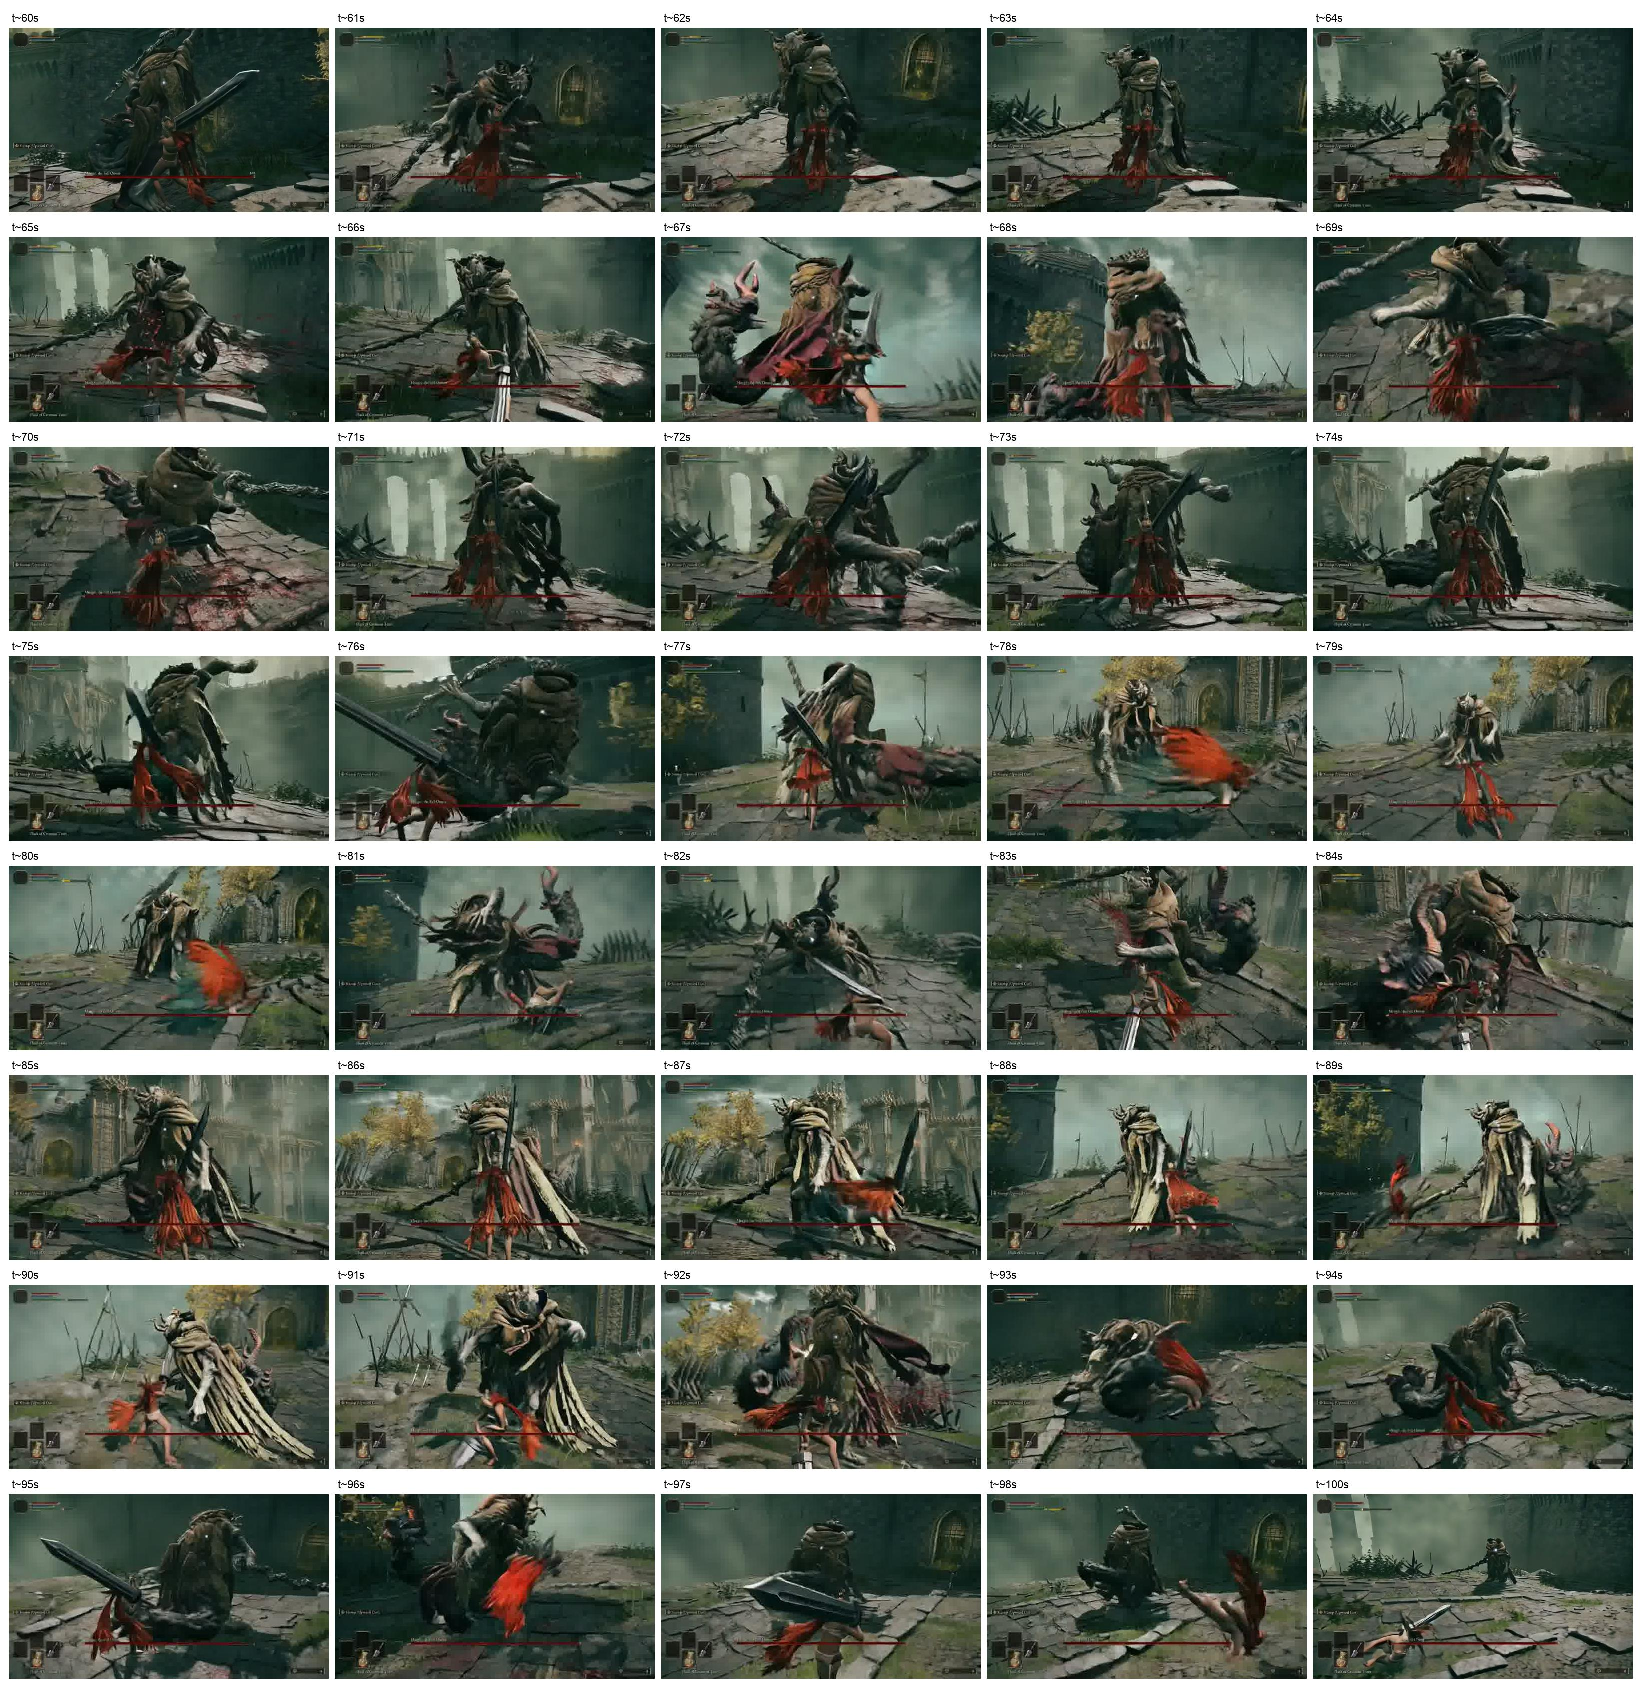
\includegraphics[width=\linewidth]{figures/margit_rollout_1min.pdf}
    \caption{\textbf{Elden Ring rollout from a continuous Margit session.}
    We show $40$ frames sampled from the generated stream starting at the $1$-minute mark.
    The sequence illustrates long-horizon visual stability and fine-grained player--boss interaction in a complex 3D adversarial scene.}
    \label{fig:margit_rollout_1min}
\end{figure}

\begin{figure}[h]
    \centering
    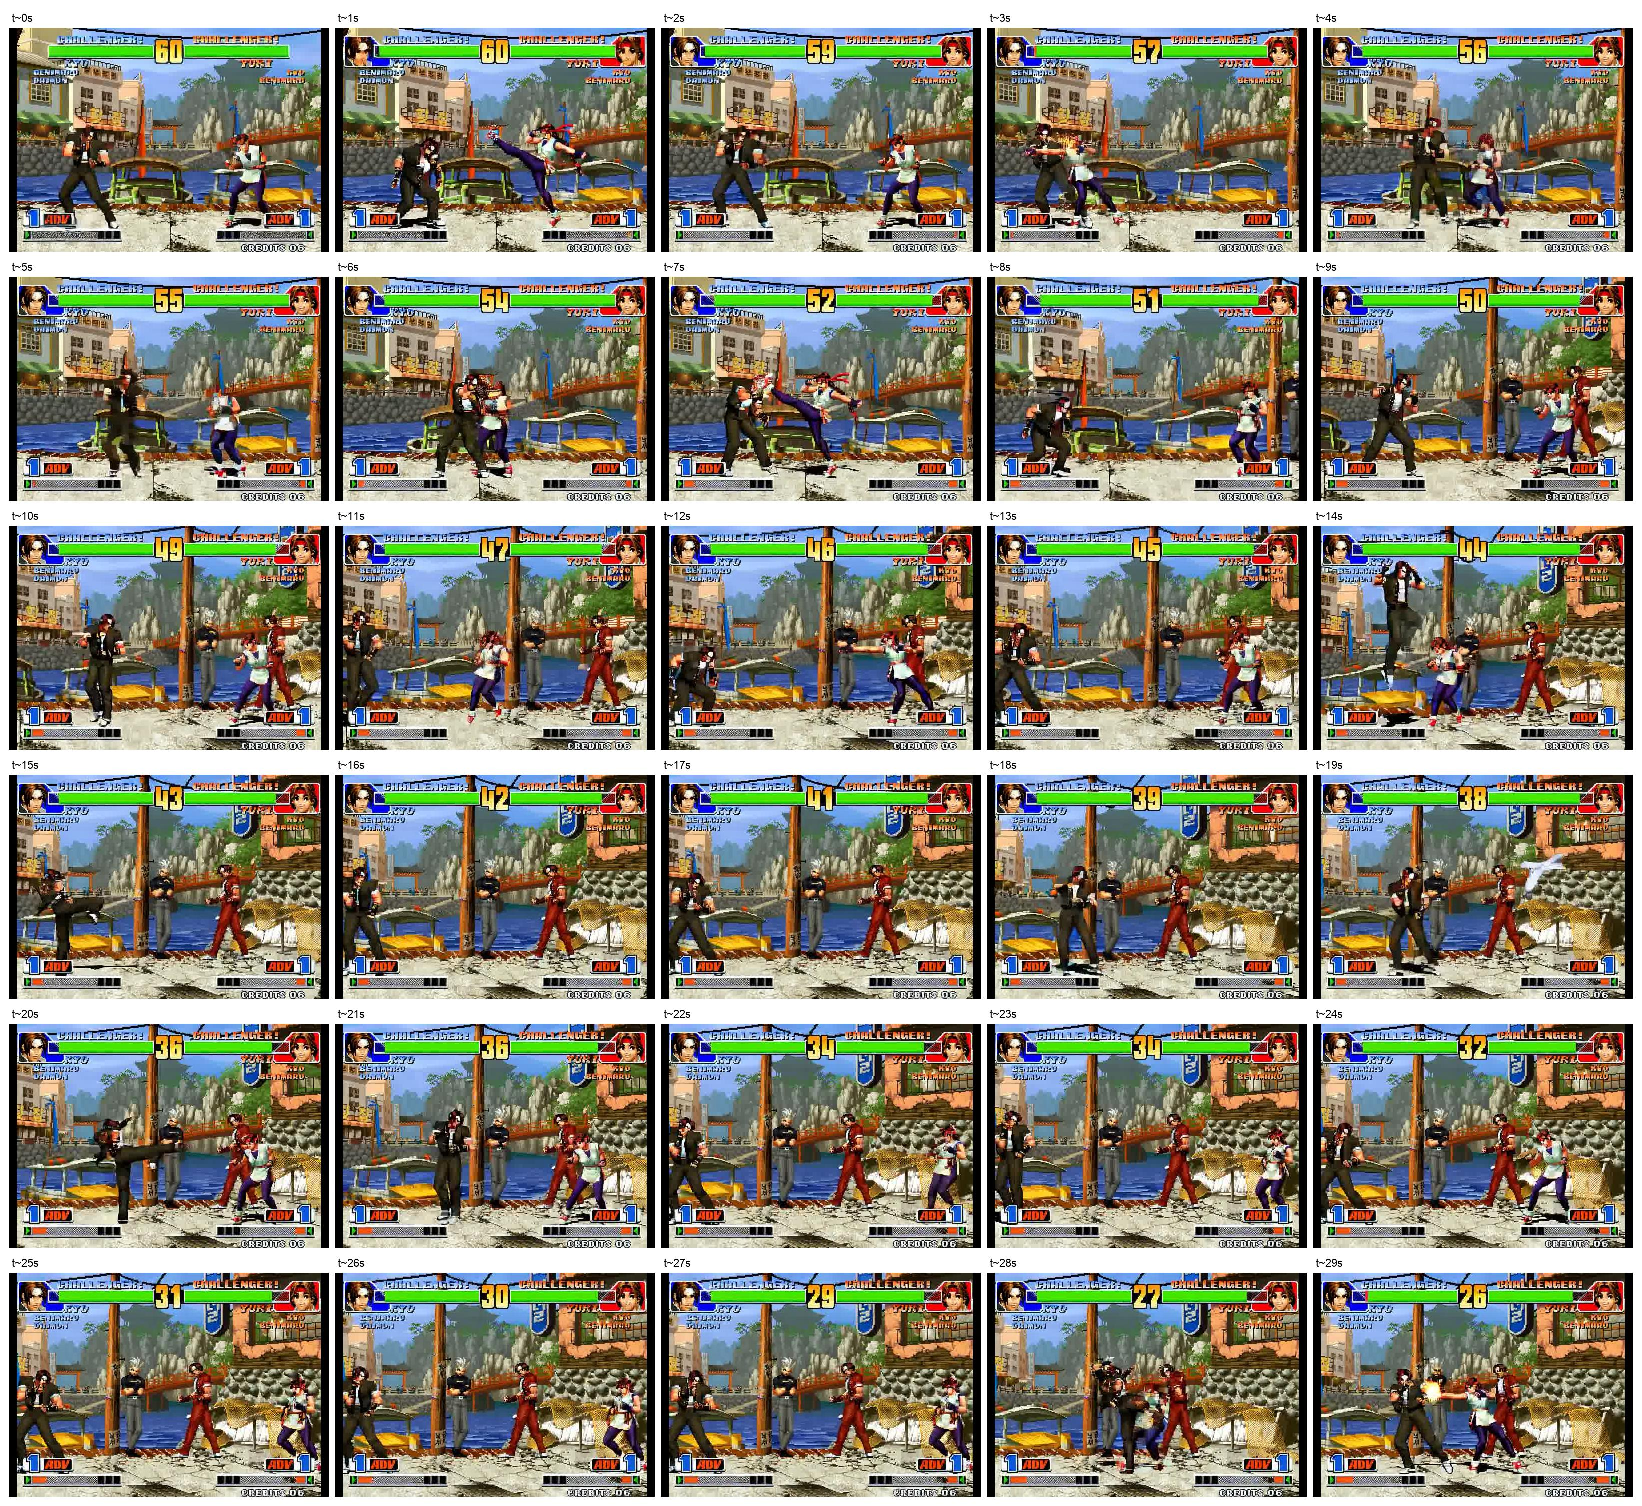
\includegraphics[width=\linewidth]{figures/kof_rollout_0.pdf}
    \caption{\textbf{KOF rollout under the same architecture and training recipe.}
    We show $30$ frames from a KOF rollout.
    The sequence illustrates that the same per-entity language-conditioning recipe also supports visually distinct 2D fighting gameplay.}
    \label{fig:kof_rollout_0}
\end{figure}
% \subsection{Additional Qualitative Results}
% \label{app:visual_results}

% We further present additional qualitative results of \methodname
% operating on the game \textit{The King of Fighters (KOF)},
% as shown in \Cref{fig:kof_demo}.
% \methodname achieves fine-grained multi-entity action control
% and accurately captures highly brief actions
% (e.g., \textit{Punching}) lasting within $0.25$\,s.

% \begin{figure*}[t]
%     \centering
%     \captionsetup{justification=raggedright, singlelinecheck=false}
%     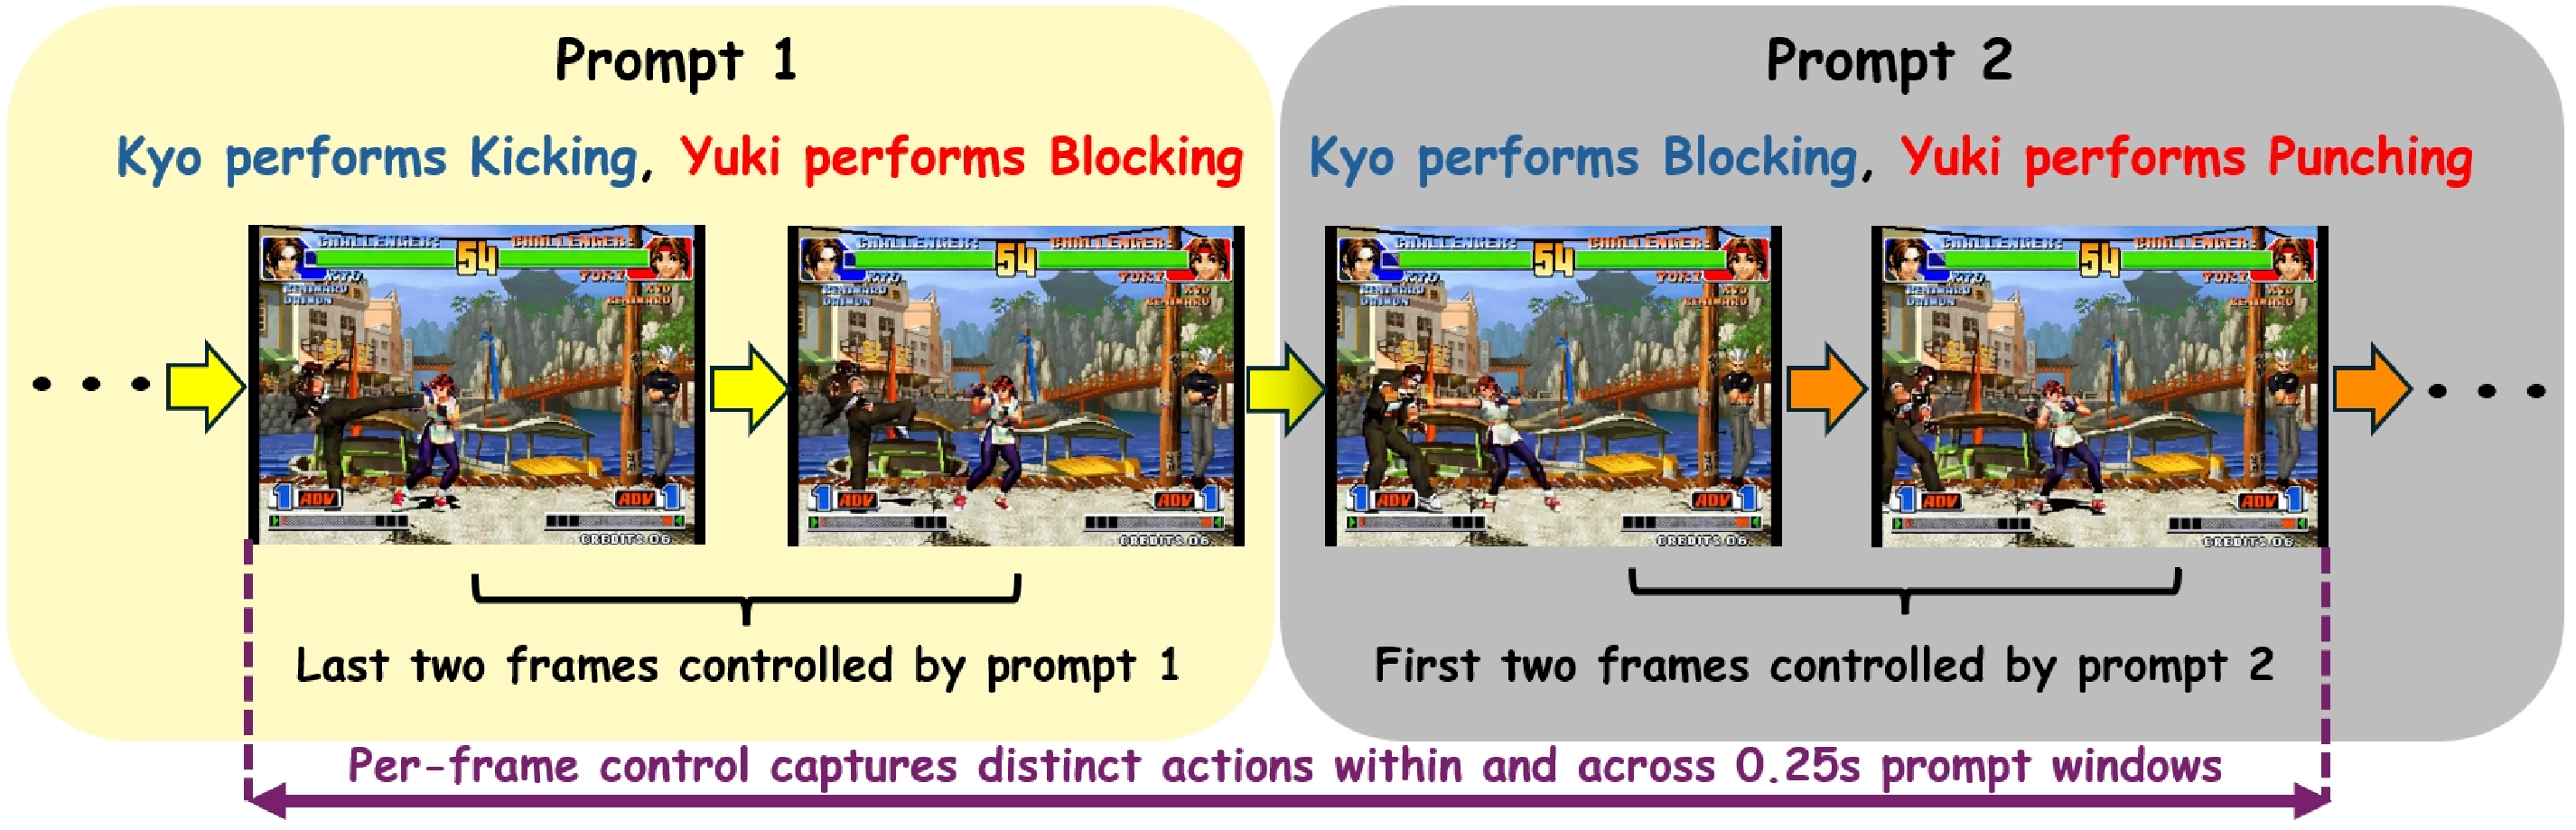
\includegraphics[width=\linewidth]{figures/fig_kof_demo.pdf}
%     \caption{\textbf{Demonstrations of fine-grained multi-entity action control of \methodname in \textit{KOF}.}
%     \methodname precisely responds to rapid action inputs and successfully captures
%     actions as brief as $0.25$\,s (e.g., \textit{Punching}),
%     demonstrating its fine-grained and responsive control capability.}
%     \label{fig:kof_demo}
% \end{figure*}

\subsection{Full Action Vocabulary}
\label{app:vocab}

We summarize the per-entity action vocabularies used for prompt conditioning in Table~\ref{tab:vocab}. The player vocabulary $\mathcal{A}_{\text{player}}$ consists of $13$ actions covering locomotion, defensive rolls, weapon attacks, and terminal states. Margit's native repertoire $\mathcal{A}_{\text{boss}}^{\text{Margit}}$ contains $30$ actions, while the Crucible Knight contributes $17$ additional non-overlapping moves. We obtain the joint boss vocabulary $\mathcal{A}_{\text{boss}}^{\text{joint}}$ with $|\mathcal{A}_{\text{boss}}^{\text{joint}}|=47$ by deduplication across the two bosses, and we adopt this joint vocabulary throughout the experiments so that any cross-entity action index is technically injectable into either boss's context.

We obtain these vocabularies by manually aggregating the raw animation-state IDs read from engine memory. The raw stream is not an action vocabulary in the human-meaningful sense: a single human action such as a heavy slash unrolls into a sequence of typically six or more consecutive raw IDs corresponding to its sub-phases (e.g., \texttt{windup}\,$\to$\,\texttt{strike}\,$\to$\,\texttt{recovery}\,$\to$\,\texttt{idle}), and a representative recording session already exposes $111$ distinct player IDs and $53$ distinct boss IDs even before the full dataset is exhausted. Domain-expert aggregation from the raw IDs to the $13$/$47$-action vocabulary is therefore a prerequisite shared by any Action-Index baseline rather than an advantage of NL conditioning, and our vocabularies define the action-level ground truth on which both NL and Action-Index baselines are evaluated. We release the full raw-ID-to-action mapping with the dataset (see Appendix~\ref{app:stronger_id} for the implications on stronger Action-Index baselines).

\begin{table}[h]
  \caption{Margit's native action vocabulary, with $|\mathcal{A}_{\text{player}}|=13$ and $|\mathcal{A}_{\text{boss}}^{\text{Margit}}|=30$. The Crucible Knight contributes additional non-overlapping actions, yielding the joint boss vocabulary $|\mathcal{A}_{\text{boss}}^{\text{joint}}|=47$ that we use throughout the experiments.}
  \label{tab:vocab}
  \centering
  \small
  \begin{tabular}{p{0.45\linewidth}p{0.45\linewidth}}
    \toprule
    \textbf{Player Actions ($\mathbf{13}$)} & \textbf{Boss Actions ($\mathbf{30}$)} \\
    \midrule
    Standing, Move ($4$dir), Roll ($4$dir), & Moving (forward\,/\,left\,/\,right), \\
    Greatsword Sweep, Greatsword Thrust, & Jump and mid-air slam, Horizontal slash, \\
    Death, Execution & Heavy overhead slash, Staff slam, \\
    & Uttering curse, Quick slam, \\
    & Double light blade throw, Staff upswing, \\
    & Tail swipe, Double light blade slash, \\
    & X-shaped slash, Charged staff thrust, \\
    & Forward charge, Jump back to disengage, \\
    & $+\,13$ additional combo/variant moves \\
    \bottomrule
  \end{tabular}
\end{table}

\subsection{Baseline Prompt Settings}
\label{app:baseline_prompt}

We specify the text prompts that we feed to the three video generation baselines compared in \Cref{fig:baseline_comparison}, namely
\textbf{Seedance~$\mathbf{2.0}$}~\citep{seedance2026seedance20advancingvideo},
\textbf{Kling~$\mathbf{3.0}$}~\citep{kuaishou2026kling}, and
\textbf{LongLive}~\citep{yang2025longlive}, as follows.

\begin{quote}
\noindent\textbf{Environment:} Stormveil Castle bridge, overcast sky, cinematic combat.\\
\textbf{Agents:} Player (Greatsword user) vs.\ Boss (Margit, the Fell Omen).
\noindent\textbf{Player:}
\begin{itemize}[noitemsep, topsep=2pt, leftmargin=1.5em]
    \item $0.00$\,s\,--\,$1.50$\,s:\; Move forward
    \item $1.50$\,s\,--\,$2.50$\,s:\; Roll forward
    \item $2.50$\,s\,--\,$3.50$\,s:\; Greatsword thrust
    \item $3.50$\,s\,--\,$4.50$\,s:\; Roll forward
    \item $4.50$\,s\,--\,$5.50$\,s:\; Greatsword thrust
    \item $5.50$\,s\,--\,$6.25$\,s:\; Roll backward
    \item $6.25$\,s\,--\,$7.25$\,s:\; Greatsword thrust
    \item $7.25$\,s\,--\,$8.00$\,s:\; Roll left
    \item $8.00$\,s\,--\,$8.75$\,s:\; Roll right
    \item $8.75$\,s\,--\,$10.00$\,s:\; Move forward
\end{itemize}
\noindent\textbf{Boss:}
\begin{itemize}[noitemsep, topsep=2pt, leftmargin=1.5em]
    \item $0.00$\,s\,--\,$2.50$\,s:\; Jump and mid-air slam
    \item $2.50$\,s\,--\,$4.00$\,s:\; Tail swipe
    \item $4.00$\,s\,--\,$5.00$\,s:\; Jump back to disengage
    \item $5.00$\,s\,--\,$7.50$\,s:\; Jump and mid-air slam
    \item $7.50$\,s\,--\,$9.00$\,s:\; Tail swipe
    \item $9.00$\,s\,--\,$10.00$\,s:\; Horizontal slash
\end{itemize}
\end{quote}

Since the three commercial baselines all incorporate built-in prompt-enhancement modules, we adopt this explicit timestamp-structured format to ensure a fair and controlled comparison with \methodname under matched per-entity action schedules.

\subsection{Experimental Setup Details}
\label{app:setup_details}
\label{app:details}

\paragraph{Why games are the testbed.}
We choose games as the testbed because the interface claim requires frame-accurate multi-entity action labels at interactive frame rates, and games are the only domain that offers all three properties simultaneously. Specifically, per-frame animation state is readable from engine memory at zero annotation cost, the action vocabularies are bounded yet non-trivial, and the evaluation criteria are unambiguous. In contrast, driving and embodied-manipulation datasets lack frame-level entity-wise annotations, and narrative-video datasets lack adversarial multi-entity dynamics.

\paragraph{Data pipeline.}
We assemble the training data from three distinct entity domains:
\begin{itemize}[leftmargin=*,topsep=2pt,itemsep=2pt]
  \item \textbf{Elden Ring -- Margit:} We collect $30$ hours of boss-fight gameplay and segment it into ${\sim}10{,}000$ high-quality $5$-second clips at $16$\,FPS after filtering and quality-based pruning, with $10\%$ held out by recording date for evaluation.
  \item \textbf{Elden Ring -- Crucible Knight:} We collect $15$ hours of comparable footage segmented and filtered identically (${\sim}5{,}000$ clips), and we use it jointly with Margit for the cross-entity evaluation.
  \item \textbf{The King of Fighters (KOF):} We collect ${\sim}5{,}000$ $60$-second fighter-pair clips at $16$\,FPS (${\approx}83$ hours in total), and we use this corpus to validate the cross-world transfer of the architecture.
\end{itemize}
For Elden Ring, we obtain all per-frame labels by reading the engine's \texttt{current\_animation} field at runtime via direct memory instrumentation, which yields zero-offset action triplets $(v_t, a_t^{\text{player}}, a_t^{\text{boss}})$ with $a_t \in \mathcal{A}_{\text{player}} \times \mathcal{A}_{\text{boss}}^{\text{joint}}$. We have $|\mathcal{A}_{\text{player}}|=13$ and $|\mathcal{A}_{\text{boss}}^{\text{joint}}|=47$, where the joint boss vocabulary is the deduplicated union of Margit and the Crucible Knight (Margit's native subset contains $30$ actions; see Appendix~\ref{app:vocab}). For KOF, we read per-frame labels from the emulator's animation-state register under the same zero-cost protocol.

\paragraph{Annotation protocol.}
For every reported ACA number, we pool all $20$ trials 
per condition ($5$ starting frames $\times$ $4$ seeds) 
across all conditions, randomly shuffle them, and have three 
annotators independently rate each clip on a three-point 
ordinal scale ($\mathbf{0}$: action absent; $\mathbf{1}$: 
partial execution; $\mathbf{2}$: full execution). 
Before rating, we strip both the conditioning-variant label 
(NL vs.\ Action-Index) and the prompt-source identity 
(in-distribution vs.\ cross-entity vs.\ OOV), so that 
all clips are rated under fully blinded conditions,
as shown in the annotation interface in \Cref{fig:annotator}. 
We take the per-trial score as the median of the three ratings, and we report ACA($\geq 1$) as the fraction of clips whose median is at least $1$.

\paragraph{Prompt-injection rollout protocol (Axes 1--3).}
We adopt the following prompt-injection protocol for all interface-evaluation rollouts in Axes 1--3, where the goal is to isolate the model's compositional steering capability:
\begin{enumerate}[leftmargin=*,topsep=2pt,itemsep=2pt,label=(\roman*)]
  \item \textbf{Starting frame.} We sample a starting frame uniformly at random from the held-out test split and decode it into the model's visual context window.
  \item \textbf{Un-conditioned warm-up.} The model then generates approximately $2$ seconds ($32$ frames) of un-conditioned video, during which we set both the player and boss action prompts to the neutral idle/standing token at every step. The model is therefore conditioned only on its own visual history. This warm-up serves two purposes. First, it places the model in a steady-state denoising regime before the prompted phase begins, which avoids the artifacts typical of cold-started rollouts. Second, it severs any residual visual cue from the test-set continuation that might otherwise inform the model that a particular action is about to occur; without this, the model could in principle reproduce the target action by extrapolating the test-set trajectory rather than by genuinely responding to the prompt.
  \item \textbf{Prompt injection.} At $t=2$\,s, we replace the neutral prompt with the target action prompt and hold it constant for the remaining $3$ seconds of the clip.
  \item \textbf{Rating.} Annotators rate the resulting $5$-second clip against the target action over the post-injection window.
\end{enumerate}
We apply the same warm-up and injection schedule to both the NL and Action-Index conditioning variants under matched starting frames and seeds, so that the interface comparison is conducted under identical visual conditions. We do not search over the warm-up duration: the $2$-second value is fixed before annotation begins.

\paragraph{Trajectory-conditioned protocol (system metrics).}
We adopt a separate trajectory-conditioned protocol for Table~\ref{tab:system} and the system-level ablations in Appendices~\ref{app:stage1_ablation} and~\ref{app:stage2_ablation}, where the goal is to measure how faithfully the model tracks a fully specified ground-truth action trajectory rather than its compositional steering ability:
\begin{itemize}[leftmargin=*,topsep=2pt,itemsep=2pt]
  \item \emph{Sample.} We use $100$ held-out $10$-second clips per model.
  \item \emph{Conditioning.} Rollouts begin at the first frame of each clip, and at every frame we set both the player and boss prompts to the ground-truth caption derived from engine memory. We use no warm-up phase and no prompt switch.
  \item \emph{Rating.} We rate each rollout as binary correct or incorrect against its source clip's action sequence, and ACA reports the fraction correct.
\end{itemize}
The two protocols therefore evaluate complementary capabilities, namely compositional steering versus trajectory fidelity, and their absolute ACA values should not be directly compared.

\paragraph{Training.}
We fine-tune the Stage~1 teacher for $51$k iterations ($1$k warmup at $256\times448$ followed by $50$k at $480\times832$) using AdamW with peak learning rate $1\times10^{-5}$ and global batch size $64$ on $16\times$H$100$ $80$\,GB GPUs. We then perform ODE initialization for $1{,}000$ steps at $480\times832$ (learning rate $5\times10^{-6}$, batch size $128$, $16\times$H$100$), followed by Self-Forcing distillation for $15$k iterations at learning rate $2\times10^{-6}$.

\paragraph{Video resolution.}
We generate all videos at $480\times832$ ($480$p) and $16$\,FPS. We compress context frames into latents through the base model's VAE at a $4\times$ spatial downsampling and a $4\times$ temporal downsampling.

\paragraph{Hit detection.}
We fine-tune Qwen3-VL-$2$B-Instruct~\citep{bai2025qwen3} with LoRA on the vision--language connector and the cross-attention modules. We aggregate frame-level predictions into a per-window classification through majority voting.

\paragraph{End-to-end throughput.}
\label{app:throughput}
We measure the diffusion student's wall-clock latency at $160$\,ms per frame on a single H100 $80$\,GB, where the per-frame loop is dominated by the diffusion pass with KV-cache sliding and RoPE decoupling, the VAE decode, and the surrounding I/O. We will release detailed per-component timings alongside the open-source code.

\begin{figure*}[t]
    \centering
    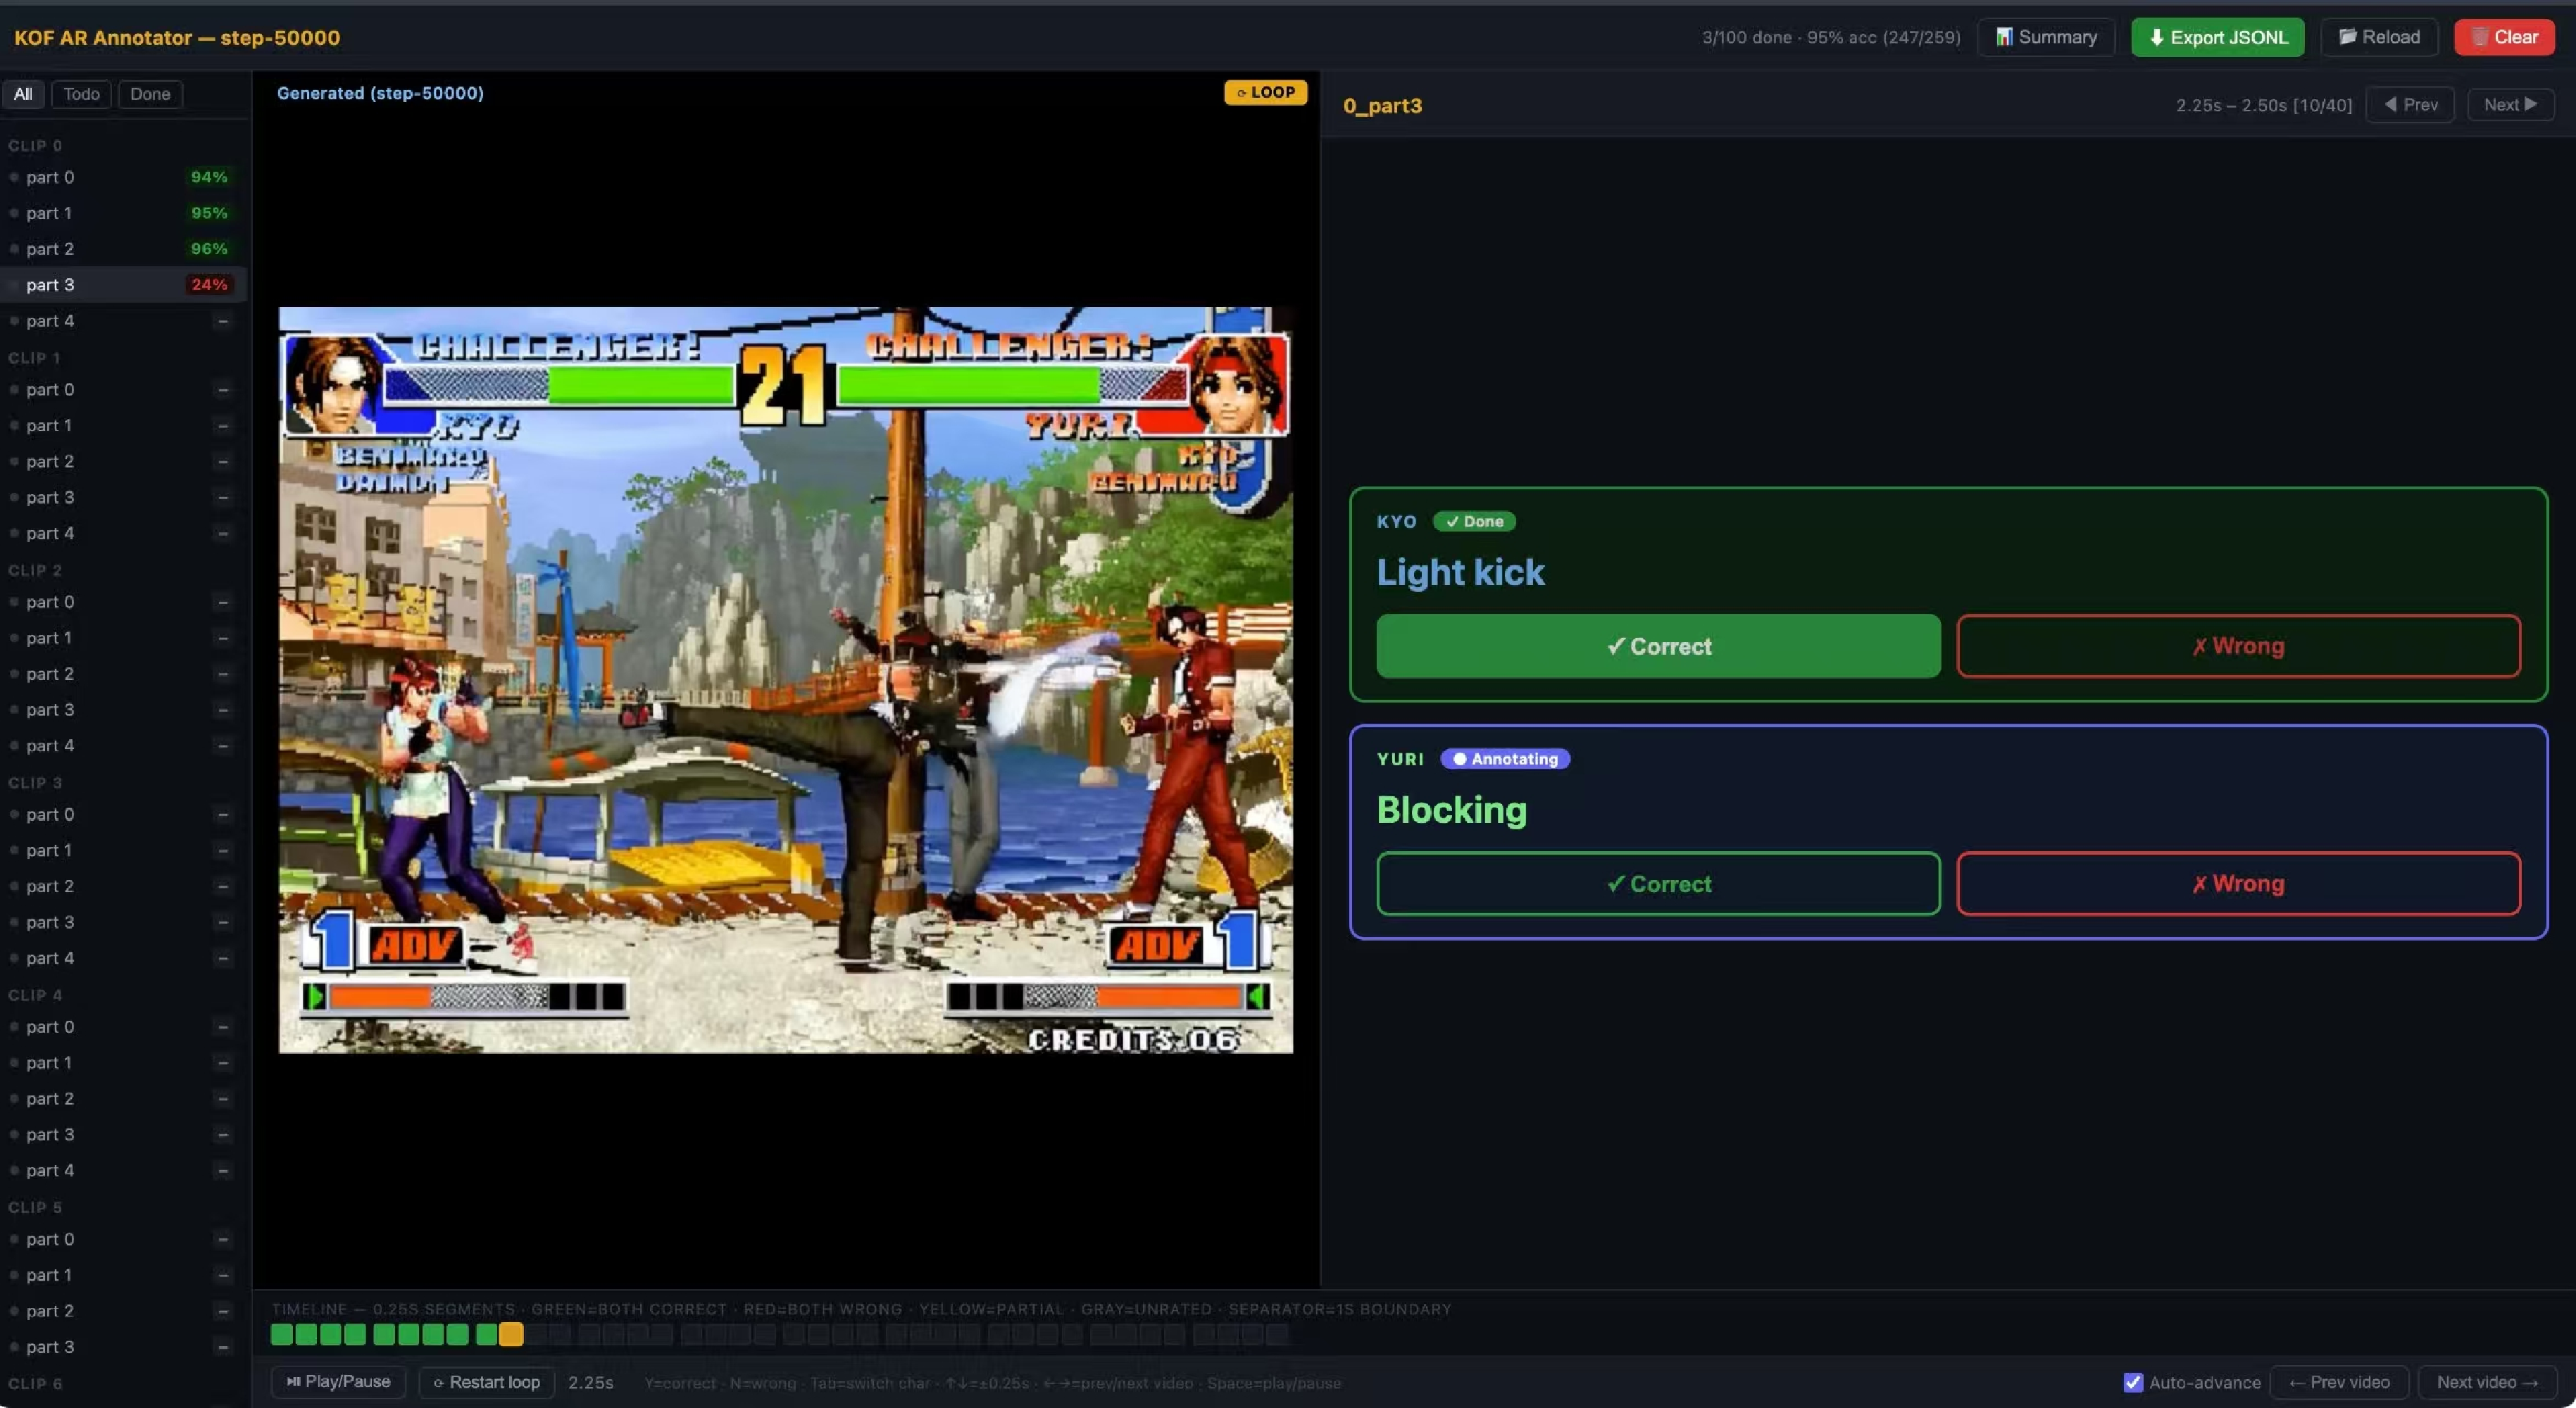
\includegraphics[width=\linewidth]{figures/fig_annotator.pdf}
    \caption{\textbf{Annotation interface for the human evaluation of Action Control Accuracy (ACA).}
    Each trial presents the annotators with a generated video clip alongside the per-entity target action label (here: \textsc{Kyo}---\textit{Light kick}; \textsc{Yuri}---\textit{Blocking}).
    We strip conditioning-variant identities (NL vs.\ Action-Index) and prompt-source labels before rating, which ensures a fully blinded evaluation.
    Each annotator rates each entity's action on the three-point ordinal scale ($\mathbf{0}$: absent; $\mathbf{1}$: partial; $\mathbf{2}$: full); we then take the per-clip ACA($\geq 1$) as the binary indicator that the median of the three ratings is at least $1$.}
    \label{fig:annotator}
\end{figure*}

\subsection{Annotator Reliability}
\label{app:reliability}

We rate $400$ generated clips in total ($200$ 
cross-entity and $200$ in-distribution) under the protocol 
of Appendix~\ref{app:setup_details}. Each clip is scored 
independently by three blinded annotators on the 
$\{0, 1, 2\}$ ordinal scale with conditioning-variant and 
prompt-source labels stripped, and we take the per-clip ACA 
score as the binary indicator that the median of the three 
ordinal ratings is at least $1$. In this subsection we 
report inter-rater consistency restricted to the $5$-pair 
cross-entity subset (the Axis~$2$ pairs in 
Table~\ref{tab:main_results}) and the $5$-action 
in-distribution subset (the Axis~$1$ actions in 
Table~\ref{tab:main_results}). 
% We exclude one candidate 
% action (m\_HorizontalSlash) from both subsets on 
% evaluation-side grounds: 
% the three-rater within-$1$ ordinal agreement on this 
% action drops to $75\%$, in clear contrast to 
% the $93$--$96\%$ range observed for all retained actions. 
% The exclusion is therefore driven by annotator reliability 
% rather than by interface behavior.

\paragraph{Within-$\mathbf{1}$ ordinal agreement.}
On the $\{0,1,2\}$ scale, raters disagree by more than one tier on fewer than $7\%$ of clips across either split. Specifically, the within-$1$ agreement on the cross-entity subset is $96.5\%$, $96.0\%$, and $95.0\%$ for the three rater pairs $A_1\!\times\!A_2$, $A_1\!\times\!A_3$, and $A_2\!\times\!A_3$; on the in-distribution subset, the corresponding numbers are $93.3\%$, $95.8\%$, and $94.2\%$. Consequently, aggregating by the median of the three ratings before binarizing at the $\geq 1$ threshold inherits a noise floor of at most one-tier disagreement on at most $7\%$ of clips, which is materially smaller than every NL\,vs.\,Action-Index gap reported in the paper.

\paragraph{Paired McNemar on cross-entity: $\mathbf{Z=6.38}$, $\mathbf{p<10^{-10}}$.}
For each (pair, starting frame, seed) triple, 
we obtain one NL clip and one Action-Index clip 
evaluated under identical visual conditioning and 
rated by the same three blinded annotators under the 
median-of-three scheme. We pool the matched triples 
across all five pairs and apply the McNemar test on the 
resulting binary scores. The test yields $49$ triples 
on which NL succeeds and Action-Index fails, against $3$ 
triples on which Action-Index succeeds and NL fails, 
giving $Z=6.38$ and $p<10^{-10}$ (one-sided). Therefore, among the clips on which the two interfaces produce different outcomes, the language interface succeeds on more than an order of magnitude as many clips as the Action-Index baseline, and the cross-entity gap cannot be attributed to cell-level fluctuation.

\subsection{Stage 1: Conditioning Architecture Ablation}
\label{app:stage1_ablation}

We ablate the two key Stage~$1$ design choices in a $2\times 2$ factorial that crosses the type of history self-attention (bidirectional vs.\ causal) with the scope of text cross-attention (noisy frame only vs.\ all frames). We train all four variants from the same Wan~$2.2$ TI2V-5B checkpoint with identical hyperparameters (batch size $64$, learning rate $2\times 10^{-5}$, resolution $256\times 448$), and we evaluate them on the held-out test split every $5$k steps up to $35$k steps under the trajectory-conditioned protocol of Appendix~\ref{app:setup_details}.

\begin{table}[h]
  \caption{\textbf{Stage~$\mathbf{1}$ architecture ablation ($\mathbf{2\times 2}$).} Each cell reports FVD$\downarrow$ at the best checkpoint, selected by the lowest FVD. $\dagger$: training never stabilizes, with FVD exceeding $1{,}100$ at all checkpoints.}
  \label{tab:ablation}
  \centering
  \setlength{\tabcolsep}{12pt}
  \begin{tabular}{lcc}
    \toprule
    & \textbf{Text: noisy only} & \textbf{Text: all frames} \\
    \midrule
    \textbf{Bidir.\ history (ours)} & $\mathbf{201.9}$ & $197.1$ \\
    \textbf{Causal history}         & $245.1$          & $1157.9^\dagger$ \\
    \bottomrule
  \end{tabular}
\end{table}

Three findings emerge from this ablation.
\textbf{($\mathbf{1}$) Bidirectional history attention consistently outperforms causal history attention} ($201.9$ vs.\ $245.1$ FVD). This confirms that forcing causal masking on history tokens breaks the bidirectional inductive bias inherited from the Wan~$2.2$ pretrained weights.
\textbf{($\mathbf{2}$) Decoupling text cross-attention to the noisy frame is essentially free} ($201.9$ vs.\ $197.1$ FVD, within noise), which demonstrates that our design preserves semantic clarity at zero quality cost.
\textbf{($\mathbf{3}$) Causal history combined with full cross-attention is unstable} (FVD $>1{,}100$ throughout training). In this configuration, injecting the current-frame action label $a_t$ into committed causal history keys contaminates those representations with future action information, which supports the temporal cross-contamination analysis in Section~\ref{sec:stage1}.
We further plot the per-step training curves in Figure~\ref{fig:ablation_curve}, and they confirm that these findings hold throughout training rather than only at a single checkpoint.

\begin{figure}[h]
\centering
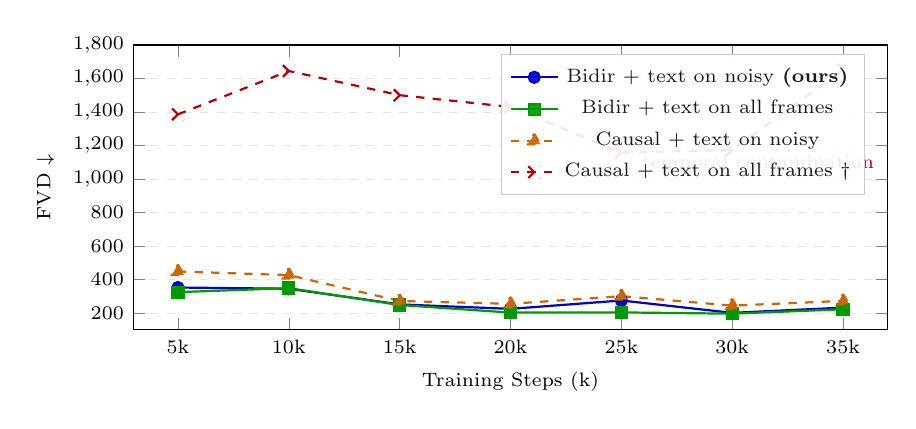
\begin{tikzpicture}[font=\small]
\begin{axis}[
  width=0.92\linewidth,
  height=5.2cm,
  xlabel={Training Steps (k)},
  ylabel={FVD $\downarrow$},
  xmin=3, xmax=37,
  ymin=100, ymax=1800,
  xtick={5,10,15,20,25,30,35},
  xticklabels={5k,10k,15k,20k,25k,30k,35k},
  ytick={200,400,600,800,1000,1200,1400,1600,1800},
  ymajorgrids=true,
  grid style={gray!20, dashed},
  legend pos=north east,
  legend style={font=\scriptsize, fill=white, fill opacity=0.9,
                draw=gray!40, inner sep=3pt, row sep=1pt},
  tick label style={font=\scriptsize},
  label style={font=\scriptsize},
  clip=true,
]
\addplot[color=blue!80!black, thick, mark=*, mark size=2pt]
  coordinates {(5,353.1)(10,345.7)(15,252.3)(20,225.7)(25,275.7)(30,201.9)(35,233.1)};
\addlegendentry{Bidir + text on noisy \textbf{(ours)}}
\addplot[color=green!60!black, thick, mark=square*, mark size=2pt]
  coordinates {(5,325.4)(10,349.4)(15,248.9)(20,203.4)(25,204.5)(30,197.1)(35,223.2)};
\addlegendentry{Bidir + text on all frames}
\addplot[color=orange!80!black, thick, mark=triangle*, mark size=2.5pt, dashed]
  coordinates {(5,448.9)(10,427.2)(15,272.7)(20,255.8)(25,301.5)(30,245.1)(35,273.3)};
\addlegendentry{Causal + text on noisy}
\addplot[color=red!70!black, thick, mark=x, mark size=3pt, dashed]
  coordinates {(5,1386.4)(10,1644.9)(15,1500.7)(20,1430.4)(25,1157.9)(30,1173.6)(35,1653.1)};
\addlegendentry{Causal + text on all frames $\dagger$}
\node[font=\scriptsize, red!70!black, anchor=west]
  at (axis cs: 25.5, 1090) {temporal contamination};
\end{axis}
\end{tikzpicture}
\caption{\textbf{Stage~$\mathbf{1}$ ablation: FVD vs.\ training steps.} Companion to Table~\ref{tab:ablation}. The causal-history plus full-cross-attention configuration ($\dagger$) collapses throughout training, whereas the other three configurations converge to FVD$\,\sim 200$.}
\label{fig:ablation_curve}
\end{figure}

\subsection{Stage 2: KV-Cache and Bounded RoPE Ablation}
\label{app:stage2_ablation}

We sweep the two Stage~$2$ 
design choices on the same 
distilled student. 
Group~A omits the bounded sliding window 
entirely and retains the full history, which incurs unbounded VRAM growth. Group~B fixes the sliding window at \texttt{kv\_window}$=7$ to match the training value $K_r=7$, and we sweep the local-RoPE cap within this group. Group~C fixes the cap at \texttt{cap}$=16$ and we sweep the window size. We report the held-out FVD under the trajectory-conditioned protocol of Appendix~\ref{app:setup_details} at both $10$\,s and $30$\,s horizons.

\begin{table}[h]
  \caption{\textbf{Stage~$\mathbf{2}$: KV-cache and RoPE ablation.} We report FVD$\downarrow$ on the $10$\,s and $30$\,s held-out test sets. $\ddagger$: full history retained in VRAM, with OOM risk on long sequences. KV sliding is the dominant factor: without it, FVD more than doubles at $30$\,s. With sliding enabled, the RoPE cap has negligible effect on FVD because the sliding window already bounds the 
  relative positions to the training range. All results are obtained using the native Wan $2.2$ VAE.}
  \label{tab:kvcache}
  \centering
  \setlength{\tabcolsep}{10pt}
  \begin{tabular}{llcc}
    \toprule
    Group & Configuration & FVD $\downarrow$ ($10$\,s) & FVD $\downarrow$ ($30$\,s) \\
    \midrule
    A: no sliding$^\ddagger$ & No cap                                 & $439.6$          & $996.9$          \\
    \midrule
    \multirow{2}{*}{B: kv$=7$}
                             & No cap                                 & $137.7$          & $141.2$          \\
                             & \textbf{cap$\mathbf{=16}$ (ours)}      & $\mathbf{138.6}$ & $\mathbf{139.2}$ \\
    \midrule
    C: cap$=16$              & kv$=4$                                 & $140.5$          & $141.9$          \\
    \bottomrule
  \end{tabular}
\end{table}

We summarize three findings.
\textbf{($\mathbf{1}$) KV sliding dominates, with benefits compounding at long horizon.}
Without sliding (Group~A), FVD rises from $439.6$ at $10$\,s to $996.9$ at $30$\,s, a $2.3\times$ degradation as the unbounded history strains memory and accumulates rollout errors. With sliding enabled (Groups~B and~C), FVD remains essentially flat across both horizons, with at most $3$ FVD points of change.
\textbf{($\mathbf{2}$) The RoPE cap has negligible empirical effect under sliding.}
The no-cap and cap$=16$ rows of Group~B differ by only $0.9$ FVD at $10$\,s and $2.0$ 
FVD at $30$\,s. The reason is that, 
under a $K_r = 7$ sliding window, the relative distance between the noisy target and any recent 
frame is bounded to $[1, 7]$ exactly by construction, 
which already covers the training range for target--recent attention.
The local-RoPE cap $C$ instead bounds the relative distance from the target to the sink frame, 
which would otherwise grow unboundedly as $p_t^{\mathrm{abs}}$ advances.
Empirically, the no-cap baseline still performs well because attention mass on the sink is small 
(the sink primarily encodes static scene anchors), so the OOD positional regime there has 
limited effect on FVD.
\textbf{($\mathbf{3}$) Window size $\mathbf{K_r=7}$ aligns with training.}
With \texttt{kv}$=4$ (Group~C), FVD stays within $3$ points of the \texttt{kv}$=7$ baseline at both horizons ($140.5$ vs.\ $138.6$ at $10$\,s; $141.9$ vs.\ $139.2$ at $30$\,s). This confirms that, once the relative-position bound is in place, the exact window length exerts only a second-order effect on quality.

\subsection{Stronger Action-Index Baselines Collapse into NL}
\label{app:stronger_id}

A natural intermediate baseline that might appear stronger than our hash-projected Action-Index interface is one whose embeddings are factorized into separate entity and action tables and initialized from a frozen text encoder such as CLIP, Qwen, or Wan's own. We argue that any such baseline is, by construction, a vocabulary-restricted special case of NL conditioning and therefore does not constitute a separate operating point. We analyze its two natural instantiations as follows.
\textbf{Frozen variant.} When we keep the text-initialized embeddings frozen, the baseline inherits exactly the pretrained semantic prior that NL exploits, and we therefore expect it to recover most of the Tier~II and Tier~III cross-entity gap. However, its inference vocabulary remains closed, so its OOV coverage on the four probes of Section~\ref{sec:language_vs_id} stays exactly $\mathbf{0}\%$. No choice of initialization can change a structural slot count.
\textbf{Trainable variant.} When we unfreeze the embeddings, the text-initialized entries specialize to their training-time entity context within a few thousand steps, and the variant is empirically dominated by the joint-vocabulary Action-Index baseline reported in Section~\ref{sec:language_vs_id}.
In either case, a factorized text-initialized Action-Index interface either collapses into NL with a hand-fixed sub-vocabulary (frozen) or reverts to the joint-vocabulary baseline (trainable).

\subsection{Axis 1: Full In-Distribution Score Distributions}
\label{app:full_indist}

We extend the main-body Axis~$1$ summary (Table~\ref{tab:main_results}) with the per-trial $2/1/0$ score distributions for both interfaces in Table~\ref{tab:indist_full}. We evaluate both NL and Action-Index on the same $20$ trials per action ($5$ starting frames $\times$ $4$ seeds), with three blinded annotators and median rating. We select the five evaluated actions as the most frequent in-distribution actions per entity, since these dominate each entity's training data and therefore provide the strongest possible supervision for the Action-Index interface, ruling out long-tail artifacts as an explanation for any subsequent NL\,vs.\,Action-Index gap.

\begin{table}[h]
  \caption{\textbf{Axis~$\mathbf{1}$ full score distributions.} Each cell reports the percentage of trials rated $\mathbf{2}$ (full execution), $\mathbf{1}$ (partial), and $\mathbf{0}$ (absent), with ACA($\geq 1$) defined as the sum of the full and partial percentages.}
  \label{tab:indist_full}
  \centering
  \setlength{\tabcolsep}{4pt}
  \begin{tabular}{lcccc}
    \toprule
    & \multicolumn{2}{c}{\textbf{NL (ours)}} & \multicolumn{2}{c}{\textbf{Action-Index}} \\
    \cmidrule(lr){2-3}\cmidrule(lr){4-5}
    Action
      & $2\,/\,1\,/\,0$\,(\%) & ACA($\geq 1$)
      & $2\,/\,1\,/\,0$\,(\%) & ACA($\geq 1$) \\
    \midrule
    Margit \textperiodcentered{} Double light blade throw
      & $60\,/\,35\,/\,\phantom{0}5$ & $\mathbf{95}$
      & $45\,/\,40\,/\,15$           & $85$            \\
    Margit \textperiodcentered{} Staff slam
      & $70\,/\,10\,/\,20$           & $\mathbf{80}$
      & $50\,/\,30\,/\,20$           & $\mathbf{80}$   \\
    Knight \textperiodcentered{} Shield block
      & $95\,/\,\phantom{0}5\,/\,\phantom{0}0$ & $\mathbf{100}$
      & $65\,/\,35\,/\,\phantom{0}0$           & $\mathbf{100}$ \\
    Knight \textperiodcentered{} Overhead slash
      & $100\,/\,\phantom{0}0\,/\,\phantom{0}0$ & $\mathbf{100}$
      & $75\,/\,10\,/\,15$                      & $85$           \\
    Knight \textperiodcentered{} Tail of the crucible
      & $70\,/\,30\,/\,\phantom{0}0$           & $\mathbf{100}$
      & $50\,/\,45\,/\,\phantom{0}5$           & $95$            \\
    \midrule
    \textbf{Mean ($\mathbf{5}$ actions)} & & $\mathbf{95}$ & & $89$ \\
    \bottomrule
  \end{tabular}
\end{table}

\subsection{Axis 2: Full Cross-Entity Distributions and Per-Tier Mechanism}
\label{app:axis2_tiers}

We extend the main-body Axis~$2$ summary (Table~\ref{tab:main_results}) with the per-trial $2/1/0$ score distributions in Table~\ref{tab:cross_entity_full}. We evaluate both interfaces on the same five cross-entity action pairs under identical annotation ($20$ trials per pair, $5$ starting frames $\times$ $4$ seeds, three blinded annotators with median rating, prompt-injection protocol of Appendix~\ref{app:setup_details}). In the rest of this subsection we first define the three tiers used to organize the pairs, and then we decompose the cross-entity NL\,vs.\,Action-Index gap by tier.

\paragraph{Definition of the three tiers.}
We grade each cross-entity action pair (source action, target entity) by the relationship between the source action and the \emph{target entity's} native action repertoire, since this relationship determines what the Action-Index interface can possibly fall back on when an out-of-context index is injected. We adopt three tiers of increasing visual overlap:
\begin{itemize}[leftmargin=*,topsep=2pt,itemsep=2pt]
  \item \textbf{Tier~$\mathbf{I}$ (no overlap):} The source action is entirely absent from the target entity's native repertoire, with no morphologically related fallback animation available. For example, the ``double light blade throw'' is exclusive to Margit and has no counterpart in the Crucible Knight's repertoire. This is the most stringent regime for the Action-Index interface, since its index-to-embedding map has no nearest neighbor to recover.
  \item \textbf{Tier~$\mathbf{II}$ (motion shared, visual style distinct):} The target entity possesses an action that shares the underlying motion class (e.g., a tail swipe) with the source action, but the two animations differ in a visually salient feature such as luminosity or trajectory shape. For instance, both Margit and the Knight execute a tail swipe, yet only the Knight's variant emits a luminous energy trail. Action-Index can fall back on the shared motion class, but it cannot produce the entity-specific visual feature.
  \item \textbf{Tier~$\mathbf{III}$ (same action label, animation alignment varies):} Both entities possess an action carrying the same lexical label (slash, overhead, horizontal), yet the underlying animations may be more or less tightly aligned in timing and amplitude. This is in principle the easiest regime for Action-Index, since its embedding can in principle map onto a visually adjacent animation.
\end{itemize}
We choose this stratification so that the three tiers progressively give the Action-Index interface more and more chance to succeed via nearest-neighbor fallback. If the cross-entity NL advantage persists across all three tiers, then the gap cannot be attributed to a single failure mode of the Action-Index interface.

\begin{table}[h]
  \caption{\textbf{Axis~$\mathbf{2}$ full score distributions.} Each cell reports the percentage of trials rated $\mathbf{2}$ (full) / $\mathbf{1}$ (partial) / $\mathbf{0}$ (absent), with ACA($\geq 1$) defined as the sum of the full and partial percentages. We grade tiers by the degree of visual overlap between the source action and the target entity's native repertoire.}
  \label{tab:cross_entity_full}
  \centering
  \setlength{\tabcolsep}{3pt}
  \begin{tabular}{llccccc}
    \toprule
    &     & \multicolumn{2}{c}{\textbf{NL (ours)}} & \multicolumn{2}{c}{\textbf{Action-Index}} \\
    \cmidrule(lr){3-4}\cmidrule(lr){5-6}
    Action prompt (source entity) & Target entity
      & $2\,/\,1\,/\,0$\,(\%) & ACA($\geq 1$)
      & $2\,/\,1\,/\,0$\,(\%) & ACA($\geq 1$) \\
    \midrule
    \multicolumn{6}{l}{\textit{Tier~$\mathbf{I}$ --- action absent from the target entity's native repertoire}} \\
    \quad Double light blade throw (Margit) & Knight
      & $65\,/\,15\,/\,20$           & $\mathbf{80}$
      & $\phantom{0}0\,/\,15\,/\,85$ & $15$           \\
    \midrule
    \multicolumn{6}{l}{\textit{Tier~$\mathbf{II}$ --- target has a morphologically similar but visually distinct action}} \\
    \quad Tail of the crucible (Knight) & Margit
      & $20\,/\,70\,/\,10$           & $\mathbf{90}$
      & $\phantom{0}0\,/\,60\,/\,40$ & $60$           \\
    \midrule
    \multicolumn{6}{l}{\textit{Tier~$\mathbf{III}$ --- both entities share a same-named action; Action-Index may fall back to it}} \\
    \quad Heavy overhead slash (Margit) & Knight
      & $95\,/\,\phantom{0}5\,/\,\phantom{0}0$ & $\mathbf{100}$
      & $60\,/\,15\,/\,25$                     & $75$           \\
    \quad Diagonal slash (Knight)       & Margit
      & $45\,/\,50\,/\,\phantom{0}5$           & $\mathbf{95}$
      & $\phantom{0}5\,/\,20\,/\,75$           & $25$           \\
    \quad Horizontal slash (Margit)     & Knight
      & $70\,/\,10\,/\,20$                     & $\mathbf{80}$
      & $\phantom{0}0\,/\,40\,/\,60$           & $40$           \\
    \midrule
    \textbf{Mean ($\mathbf{5}$ pairs)} & & & $\mathbf{89}$ & & $43$ \\
    \bottomrule
  \end{tabular}
\end{table}

\paragraph{Per-tier decomposition of the gap.}
We now expand on the cross-entity result of Section~\ref{sec:language_vs_id} by tier. We argue that the three tiers of Table~\ref{tab:cross_entity_full} together rule out every single-confounder explanation of the cross-entity gap.

\textbf{Tier~$\mathbf{I}$ (NL$=80\%$, Action-Index$=15\%$).}
We observe the largest single-pair gap of $+65$\,pp here. The Crucible Knight is never paired with the ``double light blade throw'' index during training, so this tier is also the most stringent point of the prompt-injection protocol: the cross-entity action has zero training co-occurrence with the target entity, and the un-conditioned warm-up therefore anchors the model in an arbitrary Knight pose with no preparatory frames for the requested throw, which places visual coherence and semantic compliance maximally in tension. Under this regime, the Action-Index baseline reaches only $15\%$ ACA, with all successes registering as partial rather than full execution ($0\%$ rating-$2$, $15\%$ rating-$1$). We interpret this score-distribution pattern as the intended diagnostic signature of the protocol and as consistent with an embedding-leakage account: the Margit-trained ``double light blade'' embedding does carry enough action-specific visual gradient that, when injected into Knight context, the backbone occasionally synthesizes partial luminous-blade content; however, the Knight's vocabulary contains no nearest-neighbor action that visually resembles a thrown pair of blades, so the embedding has no usable fallback, and the partial visual content fails to crystallize into a full execution. NL, in contrast, reaches $80\%$ on the same prompt, with $65\%$ rating-$2$ full executions and $15\%$ rating-$1$ partials. The reason is that ``double light blade throw'' decomposes into subword units that the text encoder has seen in many training contexts (light, blade, throw), and the compositional meaning therefore transfers to the Knight without requiring any (Knight, light-blade) training co-occurrence. The language interface thereby largely resolves the visual-coherence-versus-semantic-compliance tension that the prompt-injection protocol creates by construction. We further note that, when the same student is evaluated under the trajectory-conditioned protocol used for the system-level metrics in Table~\ref{tab:system}, where ground-truth captions accompany the visual context from frame zero and the visual--semantic tension is removed, ACA reaches $90.4$--$93.2\%$, which is the regime in which the model is actually deployed during real-time play.

\textbf{Tier~$\mathbf{II}$ (NL$=90\%$, Action-Index$=60\%$).}
We observe a $+30$\,pp gap on this tier. The source action is the Crucible Knight's luminous energy tail, while Margit possesses a structurally analogous tail-swipe action with a dark, opaque visual style. We attribute the relatively high non-zero Action-Index ACA ($60\%$) to nearest-neighbor fallback: the injected index activates Margit's existing tail motion. However, Action-Index cannot encode the luminous visual feature, since this feature is specific to the Knight's animation. NL reaches $90\%$, with $70\%$ of clips judged as partial rather than full execution. We attribute this to the fact that the prompt ``Tail of the crucible'' encodes both the motion and the luminous visual characteristic through its pretrained semantics, which suppresses Margit's native dark-tail prior. The high partial-execution rate suggests, however, that the luminous quality is rendered less crisply on Margit than on its native Knight animation in Tier~III shared-action cases.

\textbf{Tier~$\mathbf{III}$ (Action-Index$\in [25\%, 75\%]$).}
We observe that, when the source action has a same-named counterpart in the target entity's native repertoire (slash, overhead, horizontal), the Action-Index nearest-neighbor fallback is in principle the strongest, because the index-to-embedding map should land on a visually adjacent animation. Empirically, however, the fallback is sharply contingent on \emph{animation alignment} rather than on the shared label.
We illustrate this through three pairs of increasing animation mismatch.
\textit{Heavy overhead slash} is the most aligned pair, since Margit's and the Knight's overhead slashes share both timing and amplitude; Action-Index therefore reaches $75\%$ ACA, the highest cross-entity Action-Index number in the table.
\textit{Horizontal slash} carries an identical lexical label, but the two underlying animations differ in sweep duration; Action-Index drops to $40\%$.
\textit{Diagonal slash} is the most extreme case: the Knight's variant is a short jab while Margit's is a wide arcing swing, so the shared index lands on visually mismatched footage, and Action-Index falls to $25\%$. We highlight that this Tier~III value ($25\%$) is even \emph{below} the Tier~II Action-Index number ($60\%$), where at least the underlying motion class is shared. The variation across Tier~III is therefore governed by animation-level visual specificity rather than by the lexical fact that the two entities share an action name. NL, in contrast, stays above $80\%$ on all three pairs, because language conditions on motion semantics independently of which animation index the target entity happens to own. We further note the residual NL\,$\geq$\,Action-Index gap on the easiest possible Action-Index case (Heavy overhead slash, $+25$\,pp), which indicates that language provides richer steering even on unambiguous shared actions, rather than merely compensating for missing vocabulary entries.

\paragraph{Summary.}
The three tiers together rule out every single-confounder explanation of the cross-entity gap. The NL advantage is not merely that ``Action-Index has no embedding for the action'' (Tier~$\mathbf{I}$, $+65$\,pp), nor merely that ``Action-Index picks the wrong visual style'' (Tier~$\mathbf{II}$, $+30$\,pp); rather, it persists even when Action-Index has both the right embedding and the right visual style (Tier~$\mathbf{III}$, Heavy overhead slash, $+25$\,pp). We therefore conclude that the gap tracks the structural property that NL possesses and Action-Index lacks, namely the compositional decomposition of action prompts into entity-independent semantics, rather than any single failure mode of the index-bound interface.

% ather than any single failure mode of the index-bound interface.

\paragraph{VLM pairwise corroboration.}
To provide an automated sanity check complementary to the human annotation, we run a vision-language model (VLM) judge on the same five cross-entity pairs.
For each pair we uniformly sample $10$ frames from the action burst segment of each video and present all $20$ frames to \texttt{gemini-3.1-flash-lite-preview} (accessed via API), randomising which video is labelled A and which is B.
The model is prompted with the action name, a concise visual definition, and asked to (i) score each video on a $0$--$3$ action-fidelity scale and (ii) declare a winner (\textit{A}, \textit{B}, or \textit{tie}).
We repeat this for $n{=}20$ matched NL/Action-Index pairs per action and report the fraction of trials won by each interface (Table~\ref{tab:vlm_pairwise}).

\begin{table}[h]
  \caption{\textbf{VLM pairwise judge ($10$ frames per video, $n{=}20$ pairs, \texttt{gemini-3.1-flash-lite-preview}).}
    Each trial presents both videos with randomised A/B assignment; the model chooses which clip better executes the named action.
    NL win\% and ID win\% are the fractions of trials won by each interface; ties account for the remainder.
    $\Delta = \text{NL win\%} - \text{ID win\%}$.}
  \label{tab:vlm_pairwise}
  \centering
  \setlength{\tabcolsep}{6pt}
  \begin{tabular}{llccc}
    \toprule
    Tier & Action & NL win\% & ID win\% & $\Delta$ \\
    \midrule
    I   & Double light blade   & $85$ & $15$ & $+70$\,pp \\
    II  & Tail of the crucible & $50$ & $50$ & ${\approx}0$\,pp \\
    III & Heavy overhead slash & $60$ & $40$ & $+20$\,pp \\
    III & Diagonal slash       & $55$ & $45$ & $+10$\,pp \\
    III & Horizontal slash     & $60$ & $35$ & $+25$\,pp \\
    \bottomrule
  \end{tabular}
\end{table}

The VLM results largely corroborate the human annotations.
On Tier~I, the model assigns NL a $+70$\,pp advantage, consistent with the $+65$\,pp human gap and confirming the most unambiguous transfer case.
On Tier~III, NL leads by $+10$--$+25$\,pp across all three pairs, matching the human-observed pattern that Action-Index can partially fall back on a same-named animation but cannot match the steering precision of language.
The sole divergence is Tier~II (\textit{Tail of the crucible}): the VLM produces chance-level agreement ($50\%$/$50\%$), because the luminous energy tail is an out-of-distribution visual element on Margit---the VLM has no game-domain prior to distinguish it from her native golden-blade effects, and therefore cannot reliably judge which clip is correct.
This reflects an inherent limitation of general-purpose VLM judges on domain-specific cross-entity transfers: when the target action is visually OOD for the target entity, only human annotators with game context can evaluate it reliably.

\subsection{OOV Probe Set}
\label{app:oov_probes}

We evaluate four out-of-vocabulary (OOV) probes referenced in Section~\ref{sec:language_vs_id}, each obtained by editing exactly one content word of a top-$3$-by-frequency in-vocabulary base prompt. We run each probe for $10$ trials ($5$ starting frames $\times$ $2$ seeds) under the prompt-injection protocol of Appendix~\ref{app:setup_details}, and we have two annotators rate each clip on the same ordinal scale used elsewhere; ACA($\geq 1$) reports the sum of correct and partial ratings. By construction, none of the four probes corresponds to an index in the $47$-way joint vocabulary, so the Action-Index interface returns no output for any of them and its coverage is structurally $\mathbf{0}\%$, regardless of model capacity.

\begin{table}[h]
  \caption{\textbf{OOV probe results (NL).} Per-probe ACA on the four-probe evaluation set, with aggregate ACA of $\mathbf{90}\%$ over $40$ trials. Action-Index coverage on each probe is structurally $\mathbf{0}\%$.}
  \label{tab:oov_probes}
  \centering
  \setlength{\tabcolsep}{4pt}
  \begin{tabular}{llcc}
    \toprule
    Base action (entity)                & OOV prompt (edit type)                       & Trials & ACA($\geq 1$) \\
    \midrule
    Overhead slash (Knight)             & \texttt{Downward slash.} (synonym)           & $10$   & $100$            \\
    Tail of the crucible (Knight)       & \texttt{Crucible tail.} (abbreviation)       & $10$   & $100$            \\
    Shield block (Knight)               & \texttt{Shield guard.} (synonym)             & $10$   & $\phantom{0}90$  \\
    Double light blade throw (Margit)   & \texttt{Dual light blade throw.} (synonym)   & $10$   & $\phantom{0}70$  \\
    \midrule
    \textbf{Mean ($\mathbf{4}$ probes)} &                                              & $40$   & $\mathbf{90}$    \\
    \bottomrule
  \end{tabular}
\end{table}

\paragraph{Excluded probe candidates.}
We exclude two probes from the original candidate set based on setup-side issues that are upstream of the language interface itself, namely cases in which the target action is under-specified by the prompt or insufficiently distinguishable from neighboring classes by annotators. We summarize the two excluded candidates below.
\textit{\texttt{Aerial slam.}} (paraphrase of \textit{Jump and mid-air slam}) is confounded with other aerial-attack classes that share its semantic surface form. We observe that the rendered behavior disagrees with the intended target action across all $10$ trials, which indicates that the probe under-specifies the target rather than that the interface fails to act on the prompt.
\textit{\texttt{Staff swing.}} (intended as a synonym of \textit{Staff upswing}) is overly generic in Margit's repertoire, where it overlaps with \textit{Staff slam} and \textit{Charged staff thrust}; annotators report sustained ambiguity in distinguishing the intended action from these alternatives.
We therefore exclude both candidates from the quantitative aggregates rather than scoring them as ``NL failures,'' since the failure mode is upstream of the language interface itself. We release the per-trial ratings for both excluded probes alongside the codebase for transparency.

\subsection{Failure Case Analysis}
\label{app:failure}

We identify two residual failure modes of the deployed system, and we discuss each below together with its mitigation.

\textbf{($\mathbf{1}$) Rapid motion blur (rare, $<3\%$ of frames).}
We observe that, during high-speed boss attacks with extreme camera shake, the $2$-step student occasionally produces visual artifacts. We mitigate this by increasing the guidance scale to $4.5$ for frames classified as ``Boss performing leaping attack.''

\textbf{($\mathbf{2}$) Hit-detection false positives ($<5\%$ of windows).}
We observe that the VLM-based hit detector occasionally misclassifies non-damaging contact, for instance a weapon-on-shield parry, as a hit event. The rule engine tolerates such sporadic false positives because the hit-counter threshold provides natural error buffering, and the persistent state therefore remains stable over long episodes.


%% ═══════════════════════════════════════════════════════════════
\subsection{Long-Horizon Stability}
\label{app:long_horizon}

We probe whether the Self-Forcing student on Elden Ring, with its $1.75$\,s training context and RoPE-decoupled KV-cache sliding window, maintains generation quality far beyond its training horizon. To this end, we render $5$ independent rollouts of ${\sim}118$ minutes each on Margit under the trajectory-conditioned protocol of Appendix~\ref{app:setup_details}, and we evaluate FVD on $200$-second sliding windows starting at $t=30$\,min. Within each window, we extract $15$ uniformly spaced $10$-second clips per video ($5\times 15=75$ clips per window) and compare them against the held-out $10$-second test set using I$3$D features with $\textit{intersect}=\textit{False}$. We choose a window length that matches the test set's per-clip duration so that the statistics are computed on directly comparable distributions.

We report the resulting FVD trajectory in Table~\ref{tab:long_horizon}. Across the full $30$-to-$118$-minute interval, which corresponds to $88$ minutes of monitored generation per video and $27\times 75=2{,}025$ evaluated clips in total, FVD stays in $[162.4, 171.3]$ with mean $166.0$ and standard deviation $2.3$. We observe no monotonic degradation trend: the largest value ($171.3$) occurs early in the monitored interval (the $33$--$37$\,min window), and the latest window ($117$--$118.3$\,min) reads $164.5$, which is indistinguishable from the global mean. For reference, the Stage-$1$ teacher's $50$-step FVD on the same test split is $206.2$ (Table~\ref{tab:system}), so the long-horizon student stays roughly $40$ FVD points below the teacher even after running for two orders of magnitude longer than its training context.

\begin{table}[h]
  \caption{Long-horizon FVD on $5$ independent ${\sim}118$-minute Margit rollouts. Each row reports a $200$-second sliding window with $15$ uniformly sampled clips per video ($75$ clips per window, $2{,}025$ clips in total). Evaluation follows the same I$3$D protocol as Table~\ref{tab:system} on the held-out $10$-second test set.}
  \label{tab:long_horizon}
  \centering\small
  \setlength{\tabcolsep}{6pt}
  \renewcommand{\arraystretch}{0.95}
  \begin{tabular}{lc@{\hskip 1.5em}lc@{\hskip 1.5em}lc}
    \toprule
    Window (min) & FVD & Window (min) & FVD & Window (min) & FVD \\
    \midrule
    $30.0$--$33.3$   & $170.3$ & $60.0$--$63.3$   & $168.6$ & $90.0$--$93.3$    & $164.7$ \\
    $33.3$--$36.7$   & $171.3$ & $63.3$--$66.7$   & $165.1$ & $93.3$--$96.7$    & $162.4$ \\
    $36.7$--$40.0$   & $167.4$ & $66.7$--$70.0$   & $164.3$ & $96.7$--$100.0$   & $163.5$ \\
    $40.0$--$43.3$   & $168.5$ & $70.0$--$73.3$   & $164.6$ & $100.0$--$103.3$  & $165.2$ \\
    $43.3$--$46.7$   & $167.0$ & $73.3$--$76.7$   & $166.4$ & $103.3$--$106.7$  & $164.9$ \\
    $46.7$--$50.0$   & $165.9$ & $76.7$--$80.0$   & $167.7$ & $106.7$--$110.0$  & $170.3$ \\
    $50.0$--$53.3$   & $165.8$ & $80.0$--$83.3$   & $164.1$ & $110.0$--$113.3$  & $164.4$ \\
    $53.3$--$56.7$   & $166.4$ & $83.3$--$86.7$   & $163.7$ & $113.3$--$116.7$  & $165.4$ \\
    $56.7$--$60.0$   & $166.3$ & $86.7$--$90.0$   & $164.6$ & $116.7$--$118.3$  & $164.5$ \\
    \midrule
    \multicolumn{6}{c}{Aggregate over $27$ windows: mean $166.0$, std $2.3$, range $[162.4, 171.3]$.} \\
    \bottomrule
  \end{tabular}
\end{table}

We attribute this stability to the bounded RoPE-decoupled KV-cache sliding window of Section~\ref{sec:stage2}: by holding the rotary positional state inside the model's training distribution while allowing the sliding cache to attend over recent visual history, the generator avoids the positional drift that typically destabilizes long autoregressive video rollouts. This long-horizon stability also serves as the empirical foundation for the closed-loop playable system described below, which presumes that the underlying student remains visually well-behaved across multi-minute episodes.

%% ═══════════════════════════════════════════════════════════════
\subsection{Extension: Persistent Entity State via an Observer--Tracker--Policy Loop}
\label{app:persistent_state}

The two architectural patterns in the main paper (Sections~\ref{sec:stage1} and~\ref{sec:stage2}) together deliver a real-time, language-controllable video generator. However, per-frame controllability alone does not yet deliver \emph{long-horizon interactivity}. Any sufficiently long interactive video episode carries \emph{entity-level discrete state} that evolves on a substantially slower timescale than the generator's attention context, including task progress in embodied manipulation, phase state in narrative video, fuel or route state in driving, and damage and phase state in adversarial combat. Such state is not always recoverable from pixels within the current context window, is discrete rather than pixel-continuous, and must remain consistent across hundreds or thousands of frames. Standard video diffusion backbones provide no mechanism to maintain it.

We describe in this appendix an extension that addresses the gap. We present it as an extension rather than as a core contribution for three reasons: (i) the interface claim and its supporting empirical evidence stand independently of it; (ii) the instantiation is hand-specified per domain; and (iii) the loop described here is the first domain-specific instantiation rather than a fully general implementation, while a world-agnostic learned version is left as future work.

\subsubsection{The Memory Gap is Structural}
\label{app:memory_gap}

The generator attends over a bounded context of $K_s + K_r + K_n = 9$ latent tokens, spanning ${\sim}1.75$\,s of generated video through the recent window. Episode-level entity state, in contrast, evolves over minutes. The resulting ${\sim}100\times$ temporal gap cannot be closed by simply scaling the backbone: doubling the context still leaves a ${\sim}50\times$ gap, and discrete state transitions are not a quantity that video pretraining optimizes for. Empirically, we observe that a model trained on $45$ hours of Elden Ring combat data ($30$\,h Margit and $15$\,h Crucible Knight), which contains frequent player deaths and multiple boss-death sequences, never spontaneously triggers a terminal state (Section~\ref{app:neuro_eval}). The model faithfully renders every individual event, yet it never accumulates them into a state transition. We therefore conclude that this behavior is not a training-data artifact but a direct consequence of the memory-horizon mismatch.

\subsubsection{A Three-Part Loop}
\label{app:otp_loop}

We close the gap with an additive module that makes the asymmetry explicit: the neural backbone renders \emph{what the world looks like}, while an external module maintains \emph{what the world is in}. We decompose this external module into three roles, which we describe below.

\textbf{($\mathbf{1}$) Observer: structured event extraction from the generated video stream.}
We use an event extractor that operates on the rendered video itself and emits discrete, structured signals at every action window. We adopt a VLM rather than a classical detector because the extracted events are typically semantic (``did entity $E$ take damage?'', ``did task $T$ complete?'', ``did two entities collide?'') rather than low-level visual. In our instantiation, we use Qwen3-VL-$2$B-Instruct, which we fine-tune to emit a binary damage event per entity per $0.25$\,s window (Section~\ref{app:hitdet}). We emphasize that the Observer also compensates for passive-response events that we deliberately exclude from the Stage~$1$ prompt vocabulary: the generator is never conditioned to produce them, but the Observer reads them back off the rendered pixels.

\textbf{($\mathbf{2}$) Tracker: unbounded-horizon accumulation of entity state.}
We use a lightweight external state machine to aggregate the Observer's event stream into structured entity state that persists across the full episode. Unlike the bounded diffusion context, the Tracker has an unbounded temporal horizon: it integrates events from the first frame to the current frame at negligible cost. The Tracker's internal representation is typed and discrete (integer counters, categorical phase labels, or structured records), and therefore matches the actual semantics of episode-level state far more naturally than any pixel-latent representation could. In our instantiation, the Tracker maintains per-entity integer HP counters that it updates from the Observer's damage stream.

\textbf{($\mathbf{3}$) Policy: state-conditioned reinjection into the language interface.}
When the Tracker's state crosses a relevant threshold or transition condition, the Policy advances the episode to the corresponding phase and selects the next action prompt to inject into the generator. We design the Policy to be deliberately minimalist: its role is not to perform complex reasoning but to expose the Tracker's state back to the generator \emph{through the same language interface used for control}. This is what makes the loop architecturally free, since the generator sees only per-frame language prompts, regardless of whether these prompts describe user-issued actions or state-triggered transitions, and no modification to the generator is required. In our instantiation, the Policy maps HP thresholds to phase labels (normal combat, stagger, execution, terminal) and selects the corresponding prompt template.

\subsubsection{Related Work on External Memory for Generative World Models}
\label{app:external_memory_rw}

Video diffusion models operate over a bounded context window, which makes them intrinsically ill-suited to tasks that require persistent state across hundreds of frames. This limitation has motivated a family of approaches that couple neural generators with external memory.
In NLP, retrieval-augmented~\citep{lewis2020retrieval} and memory-augmented~\citep{weston2014memory} architectures delegate long-term dependencies to an explicit memory store that the neural model writes to and reads from.
In interactive world modeling, NeSyS~\citep{zhao2026nesys} constrains LLM-based simulators with executable rules to reduce hallucination, BlendRL~\citep{shindo2025blendrl} interleaves symbolic and neural policies within a single RL agent on Atari, MultiGen~\citep{po2026multigen} maintains an external memory for editable diffusion game engines, and LiveWorld~\citep{duan2026liveworld} persists entity evolution while entities are out of view.
In generative modeling more broadly, symbolic state has been injected into diffusion processes through score manipulation~\citep{scassola2025zeroshotns}, interleaved symbolic optimization~\citep{christopher2025nsd}, logic-guided vector fields~\citep{baheri2026lgvf}, and physical-consistency constraints~\citep{lin2025physar}.
Classical neuro-symbolic game AI also couples symbolic priors with neural policies~\citep{garcez2022neural, silver2016mastering, vinyals2019grandmaster}, although it operates at the policy level rather than at the generator level.
Relative to these prior approaches, our loop does not modify the generator's score, policy, or attention. It is a purely additive module that bridges the diffusion backbone's ${\sim}1.75$\,s recent context with the horizons on which entity-level discrete state actually evolves.

\subsubsection{Episode-Level State Accumulation}
\label{app:neuro_eval}

\paragraph{Protocol.}
We run independent $10$-minute test episodes and inject attack prompts at regular intervals after a calibration period. A correct system must trigger a terminal state (an entity-death sequence or execution animation) once the number of accumulated damage events crosses the per-entity threshold. We run the protocol twice under identical prompting, once with the Observer--Tracker--Policy loop attached and once without.

\paragraph{Result.}
Without the loop, no episode terminates: the neural backbone faithfully renders every individual damage animation, yet it never spontaneously transitions to a terminal sequence, since no mechanism internal to the generator can accumulate the integer count required to cross the threshold across the ${\sim}1.75$\,s local context. With the loop attached, the Tracker issues a reliable termination signal whenever its state crosses the threshold, and the Policy injects the corresponding terminal prompt back into the generator. This result directly confirms the structural prediction of Section~\ref{app:memory_gap}: the memory gap is not a training-data artifact but a backbone-horizon mismatch that cannot be closed by scaling the generator alone.

\subsubsection{Observer: VLM Event Extraction}
\label{app:hitdet}

The Observer serves as the bridge between the neural backbone's ${\sim}1.75$\,s local context and the episode-level state maintained by the Tracker. It operates on the generated video stream itself and emits a binary damage event per entity at every action window. In our instantiation the event is \emph{Taking Hit}\,/\,\emph{No Hit}, and we deploy two Observers, one per entity, using Qwen3-VL-$2$B-Instruct~\citep{qwen2024} as the backbone. We fine-tune on $4{,}477$ damage-event windows and $16{,}309$ non-event windows of $0.25$\,s each. To inject domain-specific visual priors such as blood splatters, attack contact, and stagger animations, we encode them as auxiliary instructions in the VLM prompt. To capture event-specific spatio-temporal dynamics while preserving pretrained knowledge, we update only the vision--language connector and the cross-attention modules; training completes in $8$ hours on a single H$100$.

We evaluate both Observers on a held-out test set with binary damage-event labels (Table~\ref{tab:hit_detection_eval}) and achieve over $90\%$ on every per-class Precision/Recall/F$1$ metric. We further conduct a complementary user study on distilled-generator video, and we obtain comparable numbers, which confirms robustness under the distribution shift from real to generated footage and hence under closed-loop deployment, namely the regime in which the Observer actually operates when the full loop is running.

\begin{table*}[t]
\centering
\caption{Observer evaluation (damage-event instantiation) on the held-out test set vs.\ a user study on generated video. The user-study setting matches the distribution that the Observer actually sees inside the closed loop.}
\label{tab:hit_detection_eval}
\begin{tabular}{@{}cccccc@{}}
\toprule
\textbf{Detector} & \textbf{Evaluation} & \textbf{Class} & \textbf{Precision (\%)} & \textbf{Recall (\%)} & \textbf{F$\mathbf{1}$ Score (\%)} \\ \midrule
\multirow{4}{*}{\textbf{Boss}} & \multirow{2}{*}{Test Set} & No hit     & $97.08$ & $90.01$ & $93.41$ \\
                               &                            & Taking hit & $93.50$ & $98.15$ & $95.77$ \\ \cmidrule(l){2-6} 
                               & \multirow{2}{*}{User Study}& No hit     & $87.18$ & $82.93$ & $85.00$ \\
                               &                            & Taking hit & $92.39$ & $94.44$ & $93.40$ \\ \midrule
\multirow{4}{*}{\textbf{Player}} & \multirow{2}{*}{Test Set} & No hit     & $96.01$ & $97.13$ & $96.57$ \\
                                 &                            & Taking hit & $97.02$ & $95.86$ & $96.44$ \\ \cmidrule(l){2-6} 
                                 & \multirow{2}{*}{User Study}& No hit     & $97.42$ & $92.92$ & $95.12$ \\
                                 &                            & Taking hit & $85.80$ & $94.56$ & $89.97$ \\ \bottomrule
\end{tabular}
\end{table*}

\subsubsection{Scope and Limits of This Extension}
\label{app:otp_scope}

We deliberately hand-specify the loop per domain: each domain requires its own event schema (what the Observer extracts), its own state schema (what the Tracker maintains), and its own transition table (what the Policy emits). Our current instantiation is tailored for combat, with binary damage events, integer HP counters, and HP-threshold phase transitions. Extending the loop to a new domain therefore requires re-annotating the Observer and rewriting the Tracker schema. A world-agnostic, learned version of the loop, in which all three schemas are inferred directly from event-labeled video, is an obvious next step but lies outside the scope of this paper.

\subsection{Real-Time Inference: Streaming Pipeline}
\label{app:realtime_pipeline}

Interactive deployment requires that the per-chunk generation latency not exceed the chunk's playback duration. With $C{=}2$ new latent frames per chunk and $4\times$ temporal compression at $16$\,fps, each chunk represents $500$\,ms of video; the DiT's KV-cache sliding window spans $7$ latent frames (${\sim}1.75$\,s) of attended context. On a single H100, this constraint cannot be met by a fully sequential DiT--VAE schedule; it requires overlapping the two stages in time. We describe the pipeline redesign and quantify its effect.

\subsubsection{Sequential Baseline}

In the unmodified schedule, all $N$ latent frames are produced by the DiT before VAE decoding begins. DiT and VAE thus occupy non-overlapping GPU time slots. With $C{=}2$ and the Wan backend, the per-chunk averages are $501$\,ms (DiT), $432$\,ms (VAE), and $37$\,ms (write), so the sequential pipeline processes one chunk every ${\sim}970$\,ms---a $1.94\times$ real-time ratio for the $500$\,ms of video each chunk represents.

\subsubsection{Chunk-Based Streaming}

We replace the original sequential schedule with a \emph{chunk-based producer--consumer pipeline}. Instead of generating the full latent sequence before decoding, the DiT generates latent windows incrementally and submits them to the VAE as soon as they become available. Each yielded window contains a fixed number of newly generated latent frames, optionally augmented with a small overlap of preceding latents to preserve temporal continuity across chunk boundaries.

In this mode, the DiT and VAE run on separate CUDA streams. After the DiT finishes assembling a latent window for a chunk, the host clones that window into a dedicated contiguous buffer and records a CUDA event on the DiT stream. The VAE stream waits on this event before consuming the corresponding latent buffer. This enables asynchronous GPU-side pipelining: latent generation for later chunks can overlap with VAE decoding of earlier chunks whenever hardware resources permit. The host does not impose a per-chunk global synchronization barrier, although it may occasionally wait on the oldest pending decode event to preserve ordered video emission.



\paragraph{Read-after-write hazard.}
The implementation does not expose the generator’s transient latent window directly to the VAE. Instead, each yielded latent window is materialized as a separate cloned buffer before being submitted to the decode stream. This avoids lifetime and aliasing hazards while the producer continues advancing to subsequent chunks. In other words, the VAE always consumes an immutable per-chunk latent snapshot rather than a tensor that may later be modified or discarded by the generation path.

Because each in-flight decode job owns its own latent copy, the extra memory overhead is not constant in video length but is bounded by the chunk window size and the number of queued in-flight jobs. In practice, this overhead scales with the latent window size multiplied by the queue depth limit.

\paragraph{Bounded in-flight queue.}
When the VAE is substantially faster than the DiT (e.g., with the TaeHV backend, where VAE averages $9$\,ms against DiT's ${\sim}362$\,ms), the decode queue drains near-instantly and presents no buildup risk; the bound instead guards against worst-case transient spikes or future configurations where the VAE cost approaches or exceeds the DiT cost. To prevent unbounded accumulation of pending decode jobs, we maintain a bounded FIFO queue of in-flight chunks. The producer is allowed to submit new work only while the number of pending jobs remains below a fixed queue depth \(Q\). Once the queue is full, the host dispatch loop temporarily stops submitting additional chunks until earlier decode jobs complete and are drained.

Each queued job carries its chunk index and completion event. Completed chunks are written in submission order, ensuring temporal consistency even if decode completion times vary slightly across chunks. In practice, when the VAE is much faster than the DiT, the queue remains nearly empty and the bound is rarely exercised; its primary role is to cap memory usage and provide robustness under less favorable speed ratios or transient execution spikes.

\subsubsection{Temporal Consistency}

The Wan VAE decoder is temporally convolutional: decoded pixel values at chunk boundaries depend on latents outside the chunk window. Decoding isolated chunks therefore introduces inter-chunk discontinuities. We mitigate this by prepending $L$ latent frames from the preceding chunk to each VAE input. The corresponding $L$ decoded frames are discarded after decoding; only the $C$ non-overlapping frames are retained. This is the pixel-domain analogue of the latent-domain KV-cache sliding in Section~\ref{sec:stage2}: both use a bounded overlap window to preserve causal context without unbounded history accumulation.

\subsubsection{Timing Analysis}

Each chunk of $C{=}2$ latent frames decodes to $C \times 4 = 8$ pixel frames, representing $500$\,ms of video at $16$\,FPS. We report per-chunk averages to expose stage-level costs independently of clip length; pipeline throughput is the measured active compute per chunk, directly comparable to the $500$\,ms budget.

\begin{table}[h]
  \caption{\textbf{Per-chunk pipeline timing (single H100, 2-step distilled student, $480{\times}832$, $C{=}2$, \texttt{kv\_window}{=}7, \texttt{local\_rope\_cap}{=}12).} Each chunk produces $8$ pixel frames ($500$\,ms of $16$\,FPS video). DiT and VAE columns are per-chunk averages; \emph{throughput} is measured active compute per chunk (accounting for stream overlap); \emph{Eff.\ FPS} and RT ratio are derived from throughput. Values below $1.0\times$ indicate active-compute throughput exceeds real time.}
  \label{tab:pipeline_timing}
  \centering
  \small
  \setlength{\tabcolsep}{5pt}
  \begin{tabular}{llccccr}
    \toprule
    Overlap $L$ & VAE & DiT avg (ms) & VAE avg (ms) & Throughput (ms/chunk) & Eff.\ FPS & RT ratio \\
    \midrule
    $3$ & Wan   & $501$ & $432$ & $789$ & $10.1$ & $1.58\times$ \\
    $1$ & Wan   & $504$ & $236$ & $596$ & $13.4$ & $1.19\times$ \\
    $3$ & TaeHV & $363$ & $9$ & $409$ & $19.6$ & $0.82\times$ \\
    $1$ & TaeHV & $361$ & $9$ & $406$ & $\mathbf{19.7}$ & $\mathbf{0.81\times}$ \\
    \bottomrule
  \end{tabular}
\end{table}

Three findings emerge from Table~\ref{tab:pipeline_timing}.

\textbf{(1) The Wan VAE dominates per-chunk cost.} At $L{=}3$, VAE decode averages $432$\,ms per chunk---$55\%$ of the $789$\,ms throughput. Reducing overlap to $L{=}1$ cuts the VAE cost by $45\%$ to $236$\,ms by eliminating redundant boundary decodes, lowering throughput to $596$\,ms; the pipeline remains sub-real-time ($1.19\times$).

\textbf{(2) TaeHV eliminates the VAE bottleneck.} The TaeHV lightweight decoder averages $9$\,ms per chunk regardless of $L$, reducing the VAE share to $<3\%$ of throughput. The pipeline becomes DiT-bound at ${\approx}361$--$363$\,ms/chunk (DiT), and measured throughput reaches $406$\,ms/chunk---below the $500$\,ms budget, corresponding to $19.7$\,FPS effective output at $16$\,FPS target ($0.81\times$ real-time ratio).

\textbf{(3) TaeHV reduces DiT cost.} DiT average falls from ${\sim}502$\,ms/chunk (Wan) to ${\sim}362$\,ms/chunk (TaeHV), a $28\%$ reduction. TaeHV operates in a lower-dimensional latent space, shortening the token sequence seen by the DiT attention layers and reducing the per-step cost of KV-cache construction and sliding.

Model loading (${\sim}68$--$70$\,s) and first-frame VAE encode (${\sim}0.3$--$1.6$\,s) are one-time startup costs that do not recur across chunks; in closed-loop deployment they are amortized over the full episode.

\subsection{Licenses for External Assets}
\label{app:licenses}

We list all external assets used in this work, together with their verified license terms.

\paragraph{Wan~2.2.}
We use the Wan~2.2 \texttt{TI2V-5B} variant as our Stage~1 backbone~\citep{wang2025wan}.
The model weights are released by Alibaba Group under the \textbf{Apache License 2.0}.
The full license text is available at \url{https://huggingface.co/Wan-AI/Wan2.2-TI2V-5B/blob/main/LICENSE.txt}.

\paragraph{TAEHV.}
We use TAEHV (Tiny AutoEncoder for Hunyuan Video)~\citep{BoerBohan2025TAEHV} for real-time VAE decoding during streaming inference.
TAEHV is released by Ollin Boer Bohan under the \textbf{MIT License} (Copyright \textcopyright{} 2025 Ollin Boer Bohan).
The full license text is available at \url{https://github.com/madebyollin/taehv/blob/main/LICENSE}.

\paragraph{Qwen3-VL-2B-Instruct.}
We fine-tune Qwen3-VL-2B-Instruct~\citep{bai2025qwen3} with LoRA for action annotation during dataset construction.
The model weights are released by Alibaba Cloud under the \textbf{Apache License 2.0}.
The full license text is available at \url{https://github.com/QwenLM/Qwen3-VL/blob/main/LICENSE}.

\paragraph{Elden Ring.}
\textit{Elden Ring} (\textcopyright{} 2022 Bandai Namco Entertainment Inc.\ / \textcopyright{} 2022 FromSoftware, Inc.) is a commercial video game.
All in-game footage used in this work was self-recorded for non-commercial academic research purposes, in accordance with the BANDAI NAMCO Entertainment End User License Agreement (EULA, last updated April 1, 2018).


% \subsection{Cross-Attention Spatial Routing: NL vs. Discrete Action Index}
% \label{app:routing_entropy}

% We investigate the effect of interface representation on spatial routing. Table~\ref{tab:cross_entity_full} demonstrated that NL successfully disentangles action from background during OOD entity transfer, whereas the discrete action index interface fails catastrophically, binding the action to the source entity's visual features. We trace this behavioral gap to a structural difference in representational capacity at the cross-attention layer.

% We find that the discrete action index interface is \textit{structurally deprived} of the capacity for fine-grained spatial routing. Because the action index condition consists of only two tokens (\texttt{[person\_1, boss\_1]}), when the model attends to the boss's action, the attention weights mathematically collapse into a uniform spatial distribution ($H \to H_{\text{max}}$). Conversely, the NL interface preserves fine-grained tokens (e.g., \texttt{sword}, \texttt{hand}), providing the \textit{representational capacity} to evolve specific attention heads that execute localized spatial routing ($H \ll H_{\text{max}}$). 

% To prove this, we measure the micro-level routing capacity.

% \paragraph{Probe: Microscopic Representational Capacity (Best Head $H$).}
% We measure the spatial entropy of the attention weights at the ``best head''---the specific layer and head chosen to maximize attention mass on the action tokens. The theoretical ceiling is $H_{\max} = \log(1560) \approx 7.3524$ nats, attained when attention is uniformly broadcast over every spatial patch.

% \begin{table}[h]
%   \caption{\textbf{Spatial entropy of best-head cross-attention routing, per action.}
%     $H$ is measured at the layer-head pair with highest attention concentration on the action token; ceiling $H_{\max}{=}7.352$ nats.
%     $\Delta H{=}H_{\text{OOD}}{-}H_{\text{IDist}}$ under a Margit$\to$Knight context swap.
%     Action index entropy is identical across all 10 actions and both contexts to floating-point precision, and is reported once.}
%   \label{tab:routing_entropy}
%   \centering\small
%   \setlength{\tabcolsep}{5pt}
%   \begin{tabular}{llccc}
%     \toprule
%     Action (GID) & Keyword & $H_{\text{NL,IDist}}$ & $H_{\text{NL,OOD}}$ & $\Delta H_{\text{NL}}$ \\
%     \midrule
%     Double light blade throw (34) & blade & 6.218 & 5.721 & $-$0.50 \\
%     Double light blade slash (44) & blade & 5.625 & 6.415 & $+$0.79 \\
%     Double light blade upswing(54) & blade & 6.489 & 6.139 & $-$0.35 \\
%     Quick slam (42) & slam & 6.365 & 6.651 & $+$0.29 \\
%     Light hammer slam (63) & slam & 6.862 & 6.842 & $-$0.02 \\
%     Heavy overhead slash (32) & slash & 7.075 & 7.072 & $-$0.003 \\
%     Double horizontal slash (46) & slash & 7.063 & 7.065 & $+$0.002 \\
%     X-shaped slash (53) & slash & 7.055 & 7.055 & $-$0.001 \\
%     Overhead+horizontal combo (55) & slash & 7.076 & 7.080 & $+$0.004 \\
%     Light blade thrust (64) & thrust & 7.069 & 7.074 & $+$0.005 \\
%     \midrule
%     \textbf{Mean (10 actions)} & & \textbf{6.690} & \textbf{6.711} & $\mathbf{+0.02}$ \\
%     \midrule
%     \multicolumn{2}{l}{\textbf{Action Index (all 10 actions, both contexts)}} &
%     \multicolumn{3}{c}{$H = 7.352 = H_{\max}$;\quad $\Delta H < 10^{-11}$} \\
%     \bottomrule
%   \end{tabular}
% \end{table}

% As shown in Table~\ref{tab:routing_entropy}, across 10 compound actions, the action index interface yields a best-head spatial entropy strictly equal to the ceiling ($H_{\text{index}} = 7.3524$, with concentration ratio $\rho=2.000$). This is a mathematical inevitability: because $S_k=2$, maximizing attention on the boss slot forces the softmax distribution to assign a weight of $1.0$ to \texttt{boss\_1} for every single spatial patch, resulting in an absolutely flat spatial distribution. The action index interface is structurally incapable of routing.

% In contrast, the NL interface evolves specific heads that route fine-grained tokens locally. Across the same 10 actions, the NL best-head spatial entropy averages $H_{\text{NL}} \approx 6.69$, sitting consistently below the ceiling. The model successfully routes specific semantic tokens (like \texttt{blade} or \texttt{slash}) to the relevant spatial regions, and this routing structure remains stable under entity shift ($\Delta H_{\text{NL}} = +0.02$ on average).

% \paragraph{Implication.}
% The failure of the discrete action index interface is rooted in structural collapse: because $S_k=2$, it is forced to compress the entity, action, and weapon into a single entangled vector. The probe proves this vector cannot be spatially routed, and is instead globally broadcast. Consequently, the downstream self-attention layers receive a globally entangled signal and cannot disentangle the action from the source entity's background.

% The success of the NL interface stems from its representational capacity. Its fine-grained tokens provide the structural foundation to maintain sub-ceiling, entity-stable routing cues in specific heads. When the self-attention layers process the injected context, they leverage these micro-level routing cues to correctly bind the action to the target entity without polluting the background, enabling successful OOD generalization.

